\documentclass[11pt]{extarticle} 
%% https://tex.stackexchange.com/questions/528831/why-doesnt-the-bm-package-work-with-the-unicode-math-package
\usepackage{unicode-math}
%\usepackage{mathrsfs}
\usepackage{amsthm,graphicx,xcolor,natbib,enumitem,booktabs,tabularx}
\usepackage[paperwidth=126mm,paperheight=96mm,top=5mm,bottom=5mm,right=5mm,left=5mm]{geometry}
\pagenumbering{gobble}

\usepackage[BoldFont,SlantFont]{xeCJK}  
\xeCJKsetemboldenfactor{2}
\setCJKmainfont{cwTeX Q Yuan Medium}

\usepackage{hyperref}
\hypersetup{
    colorlinks,
    linkcolor={red!50!black},
    citecolor={blue!60!black},
    urlcolor={blue!60!black}
}

\newcommand{\ds}{\displaystyle}
\newcommand{\ie}{\;\Longrightarrow\;}
\newcommand{\ifff}{\;\Longleftrightarrow\;}
\newcommand{\mi}{\mathrm{i}}
\DeclareMathOperator*{\dom}{dom}
\DeclareMathOperator*{\codom}{codom}
\DeclareMathOperator*{\ran}{ran}
\newcommand{\floor}[1]{\lfloor #1 \rfloor}
\newcommand{\ceil}[1]{\lceil #1 \rceil}
\newcommand{\Set}[2]{\big\{ \ #1\ \big|\ #2\ \big\}}
\newcommand{\pdiff}[2]{\frac{\partial\hfil#1\hfil}{\partial #2}}
\newcommand{\vf}{\symbfup{f}}
\newcommand{\vx}{\symbfup{x}}
\newcommand{\vw}{\symbfup{w}}
\newcommand{\vd}{\symbfup{d}}
\newcommand{\vg}{\symbfup{g}}
\newcommand{\vH}{\symbfup{H}}
\newcommand{\vb}{\symbfup{b}}
\newcommand{\vy}{\symbfup{y}}
\newcommand{\vW}{\symbfup{W}}
\newcommand{\vbb}{\symbfup{\beta}}

\DeclareMathOperator\prb{{\sf P}}
\DeclareMathOperator\expc{{\sf E}}
\DeclareMathOperator\var{var}
\DeclareMathOperator\cov{cov}
\DeclareMathOperator\cor{cor}
\DeclareMathOperator*{\argmax}{\arg\!\max}
\DeclareMathOperator*{\argmin}{\arg\!\min}
\DeclareMathOperator*{\im}{Im}
\DeclareMathOperator*{\re}{Re}
\DeclareMathOperator*{\conv}{conv}
\DeclareMathOperator*{\proj}{proj}
\DeclareMathOperator*{\tr}{tr}
\DeclareMathOperator*{\diag}{diag}
\DeclareMathOperator*{\epi}{epi}
\DeclareMathOperator*{\dist}{dist}
\DeclareMathOperator*{\inte}{int}
\DeclareMathOperator*{\relint}{relint}

\theoremstyle{definition}
\newtheorem*{dfn}{Definition}
\newtheorem*{prp}{Property}
\newtheorem*{thm}{Theorem}
\newtheorem*{ex}{Example}
\newtheorem*{sol}{Solution}
\newtheorem*{prf}{Proof}

\newcommand\scalemath[2]{\scalebox{#1}{\mbox{\ensuremath{\displaystyle #2}}}}

%%%%%%%%%%%%%%%%%%%%%%%%%%%%%%%%%%%%%%%%%%%%%%%%%%%%%%%%%%%%%%%%%%%%%%%%%%%%%
% Packages
%\usepackage{fullpage}
%\usepackage{import}
\usepackage{subfigure}
%\usepackage{authblk}
%\usepackage{xr-hyper}       % cross-referencing
\usepackage{url}            % simple URL typesetting
%\usepackage{nicefrac}       % compact symbols for 1/2, etc.
%\usepackage{microtype, comment}      % microtypography
\usepackage{soul, multirow, caption, comment, amsthm, adjustbox, dsfont}
%\usepackage[shortlabels]{enumitem}
%\usepackage{lineno}
\usepackage{algorithm2e}[ruled]
%\usepackage[normalem]{ulem}
%\usepackage[left]{showlabels}

% user defined colors
\definecolor{darkred}{rgb}{0.55, 0.0, 0.0}
\definecolor{darkgreen}{rgb}{0.0, 0.55, 0.0}
\definecolor{darkblue}{rgb}{0.0, 0.0, 0.55}

\newcommand{\aaotodr}[1]{{\textcolor{blue}{(@Deep:#1)}}}  %comments by Assad
\newcommand{\drtoaao}[1]{{\textcolor{red}{(@Assad:#1)}}} %comments by Deep
\newcommand{\drcorr}[2]{{\textcolor{blue}{\sout{#1}{#2}}}} %corrections by Deep
\newcommand{\opcorr}[2]{{\textcolor{cyan}{\sout{#1}{#2}}}} %corrections by Orazio

% This just formats it nicely
%\renewcommand{\showlabelsetlabel}[1]{
%\mbox{\parbox[t]{\marginparwidth}{\raggedleft\normalfont\small\ttfamily\color{blue}#1}}} 

% Variables and fields
\newcommand{\x}{\symbfup{x}}  
\newcommand{\X}{\symbfup{X}}
\newcommand{\z}{\symbfup{z}}
\newcommand{\Z}{\symbfup{Z}}
\newcommand{\s}{\symbfup{s}}                    
\newcommand{\y}{\symbfup{y}}            
\newcommand{\Y}{\symbfup{Y}}  	   
\newcommand{\W}{\symbfup{W}}   	       
\newcommand{\bb}{\symbfup{b}}        	          
\newcommand{\btheta}{\symbfup{\theta}}
\newcommand{\f}{\symbfup{f}} 
\newcommand{\Hp}{\symbfup{\Theta}} 
\newcommand{\g}{\symbfup{g}}
\newcommand{\G}{\symbfup{G}}
\newcommand{\V}{\symbfup{V}}

% Spaces
\newcommand{\Ro}{\mathbb{R}}           	                % real line
\newcommand{\bigO}{\mathcal{O}}

% Maps and functions
\newcommand{\gen}{\symbfup{g}}       	                % generator
\newcommand{\disc}{d}                 		        % discriminator
\newcommand{\loss}{\mathcal{L}}     	                % loss function

% Distributions
\newcommand{\pinfv}{p_\mathcal{X}}           		% distribution of inferred field
\newcommand{\priorinfv}{p_\mathcal{X}^\text{prior}}     % prior distribution of inferred field
\newcommand{\pginfv}{p_\mathcal{X}^\text{g}}            % distribution of inferred field induced by the generator
\newcommand{\postinfv}{p_\mathcal{X}^\text{post}}       % posterior distribution of inferred field
\newcommand{\mcmcinfv}{p_\mathcal{X}^\text{MCMC}}       % posterior MCMC distribution of inferred field
\newcommand{\plsv}{p_\mathcal{Z}}            	    	% distribution of latent space vector
\newcommand{\priorlsv}{p_\mathcal{Z}^\text{prior}}      % prior distribution of latent space vector
\newcommand{\postlsv}{p_\mathcal{Z}^\text{post}}        % posterior distribution of latent space vector
\newcommand{\pmeas}{p_\mathcal{Y}}                      % probability of evidence
\newcommand{\plike}{p_\mathcal{Y}^\text{like}}          % likelihood
\newcommand{\pn}{p_\eta}             		        % distribution of noise

% Operators
\newcommand{\ud}{{\text{d}}}
\newcommand{\df}[2]{\frac{\partial #1}{\partial #2}}
\newcommand{\dd}[2]{\frac{\ud #1}{\ud #2}}
%\newcommand{\ex}[2]{\underset{#1}{\mathbb{E}}\left[ #2\right]}
%\newcommand{\var}[2]{\underset{#1}{\text{Var}}\left[ #2\right]}
\newcommand{\bO}{\mathcal{O}}
\DeclareMathOperator*{\amin}{\rm{\arg \min}}
\DeclareMathOperator*{\amax}{\rm{\arg \max}}

\newtheorem{theorem}{Theorem}%[section] 
\newtheorem{example}{Example}%[section] 
\newtheorem{question}{Question}%[section] 
\newtheorem{remark}{Remark}%[section] 
\newtheorem{corollary}{Corollary}%[section]
\newtheorem{assumption}{Assumption}%[section]

%%%%%%%%%%%%%%%%%%%%%%%%%%%%%%%%%%%%%%%%%%%%%%%%%%%%%%%%%%%%%%%%%%%%%%%%%%%%%

\begin{document}
\title{\texorpdfstring{\vspace{15mm} Operations Research\\ 10. Neural Network (NN)}{Operations Research\\ 10. Neural Network (NN)}} 
\author{}
\date{}
\maketitle

\newpage

\section*{MLP / NN Architecture}

\begin{itemize}\setlength{\itemsep=0pt}
  \item The objective: Using an \textbf{MultiLayer Perceptron} (MLP) / \textbf{Neural Network} (NN), denoted as $\mathcal{F}$, to approximate a function $\vf:\vx\in\Ro^d\to\vy\in\Ro^D$ 
  \item Computing units of an MLP / NN, called \textbf{artificial neurons}, are stacked in a number of consecutive layers
  \item The zeroth layer of $\mathcal{F}$ is called the \textbf{source layer}, which is not a computing layer but is only responsible for providing an input (of dimension $d$) to the network
  \item The last layer of $\mathcal{F}$ is called the \textbf{output layer}, which outputs the network's prediction of dimension $D$
  \item Every other layer in between is called a \textbf{hidden layer}; the number of neurons in a layer defines the \textbf{width} of that layer
\end{itemize}
A schematic of an MLP / NN with 2 hidden layers is shown in Figure \ref{fig:MLP}. 

\begin{figure}[htbp]
  \begin{center}
    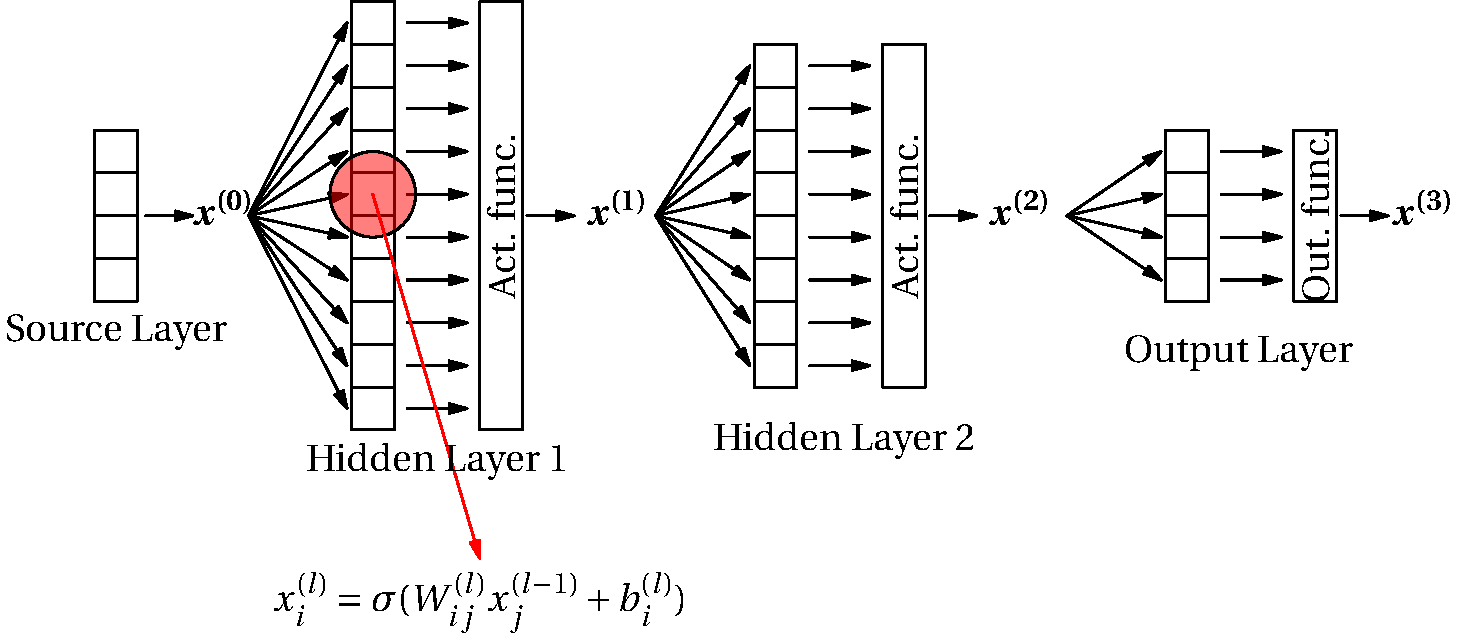
\includegraphics[width=0.9\textwidth]{fig/nn/MLP.pdf}
    \caption{MLP / NN with 2 hidden layers}
    \label{fig:MLP}
  \end{center}
\end{figure}

\newpage

\section*{Operations in MLP / NN}

\begin{itemize}%\setlength{\itemsep=0pt}
  \item Consider a MLP / NN of $L$ hidden layers, with the width of layer $(l)$ denoted as $H_l$, $\forall\,l=0,\,1,\,...,\,L+1$ 
  \item For consistency with $\vf$ that we are trying to approximate, we must have $H_0 = d$ and $H_{L+1} = D$
  \item The output vector for $l$-th layer is denoted by $\vx^{(l)}\in\Ro^{H_l}$, which will be the input to the next layer
  \item Set $\vx^{(0)} = \vx\in\Ro^d$, which will be the input signal provided by the input layer
  \item In each layer $l$, $1 \leqslant l \leqslant L+1$, the $i$-th neuron performs an affine transformation on that layers input $\vx^{(l-1)}$ followed by a non-linear transformation
    \begin{equation*}
      x_i^{(l)} = \sigma\Big(\underbrace{W^{(l)}_{ij} x_j^{(l-1)} }_{\text{Einstein sum}}+ b^{(l)}_i\Big), \quad 1 \leqslant i \leqslant H_l, \quad 1 \leqslant j \leqslant H_{l-1}
    \end{equation*}
  \item $W^{(l)}_{ij}$, $b^{(l)}_i$: the \textbf{weights} and \textbf{bias} associated with $i$-th neuron of layer $l$
  \item $\sigma(.)$: the \textbf{activation function} which plays a pivotal role in helping the network to represent non-linear complex functions
  \item Set $\vW^{(l)} \in \Ro^{H_{l-1} \times H_{l}}$ to be the weight matrix for layer $l$ and $\vb^{(l)} \in \Ro^{H_l}$ to be the bias vector for layer $l$, one can rewrite the action of the whole layer as
    \begin{equation}
      \vx^{(l)} = \sigma\left(\mathcal{A}^{(l)}(\vx^{(l-1)})\right), \quad \mathcal{A}^{(l)}(\vx^{(l-1)}) = \vW^{(l)} \vx^{(l-1)}+ \vb^{(l)}
    \end{equation}
    where the activation function is applied component-wise 
  \item The action of the network $\mathcal{F}: \Ro^d \mapsto \Ro^D$ can be seen as a composition of alternating affine transformations and component-wise activations
    \begin{equation}
      \mathcal{F}(\vx) = \mathcal{A}^{(L+1)} \circ \sigma \circ \mathcal{A}^{(L)} \circ  \sigma \circ \mathcal{A}^{(L-1)} \circ \cdots  \circ \sigma \circ \mathcal{A}^{(1)} (\vx).
    \end{equation}

%We make a few remarks here:
%\begin{enumerate}
%  \item For simplicity of the representation, we assume that the same activation function is used across all layers of the network. However, this is not a strict rule. In fact, there is recent evidence that suggests that alternating activation function from layer to layer leads to better neural networks \cite{Yarotsky2021}.
%  \item At times, there might be an output function $O$ instead of an activation function at the end of the output layer, which is typically used to reformulate the output into a suitable form. We will see examples of such functions later in the course.
%  \item We will use the term \textbf{depth} of the network to denote the number of computing layers in the MLP, i.e. the number of hidden layers and the output layer, which would be $L+1$ as per the notations used above.
%\end{enumerate}

  \item The parameters of the network is all the weights and biases, which will be denoted as $\ds\btheta = \{\vW^{(l)}, \vb^{(l)} \}_{l=1}^{L+1} \in \Ro^{N_\theta}$, where $\ds N_\theta = \sum_{l=1}^{L+1} (H_{l-1} + 1) H_l$ denotes the total number of parameters of the network 

  \item The network $\mathcal{F}(\vx; \btheta)$ represents a family of parameterized functions, where $\btheta$ needs to suitably chosen such that the network approximates the target function $f(\vx)$ at the input $\vx$

\end{itemize}

%\begin{question}
%  Prove that $\ds N_\theta = \sum_{l=1}^{L+1} (H_{l-1} + 1) H_l$.
%\end{question}

\newpage

%\section*{Activation Functions}
%The activation function is perhaps the most important component of an MLP. A large number of activations are available in literature, each with its own advantages and disadvantages. Let us take a look at a few of these options (also see Figure \ref{fig:actfunc}).

\begin{figure}[htbp!]
  \begin{center}
    \subfigure[Linear]{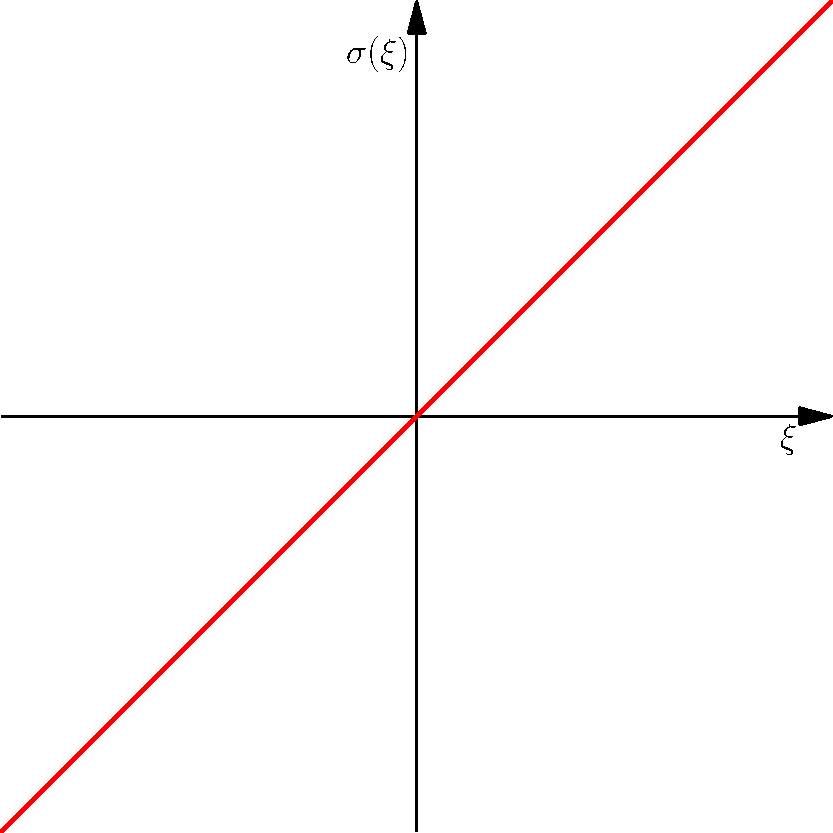
\includegraphics[width=0.25\textwidth]{fig/nn/linear.pdf}}
    \subfigure[ReLU]{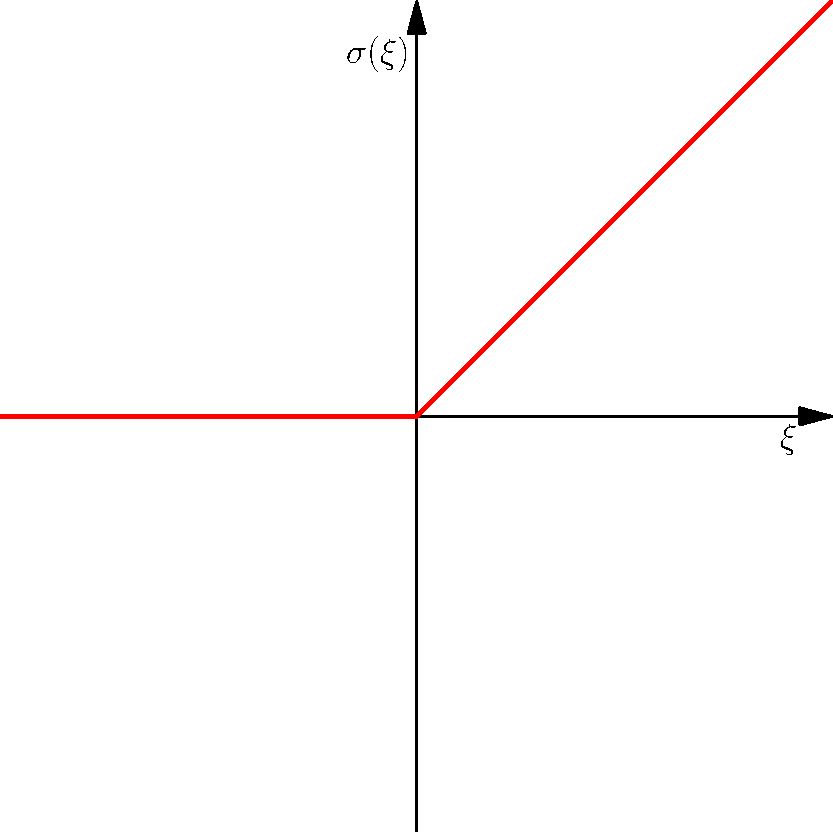
\includegraphics[width=0.25\textwidth]{fig/nn/relu.pdf}}
    \subfigure[Leaky ReLU]{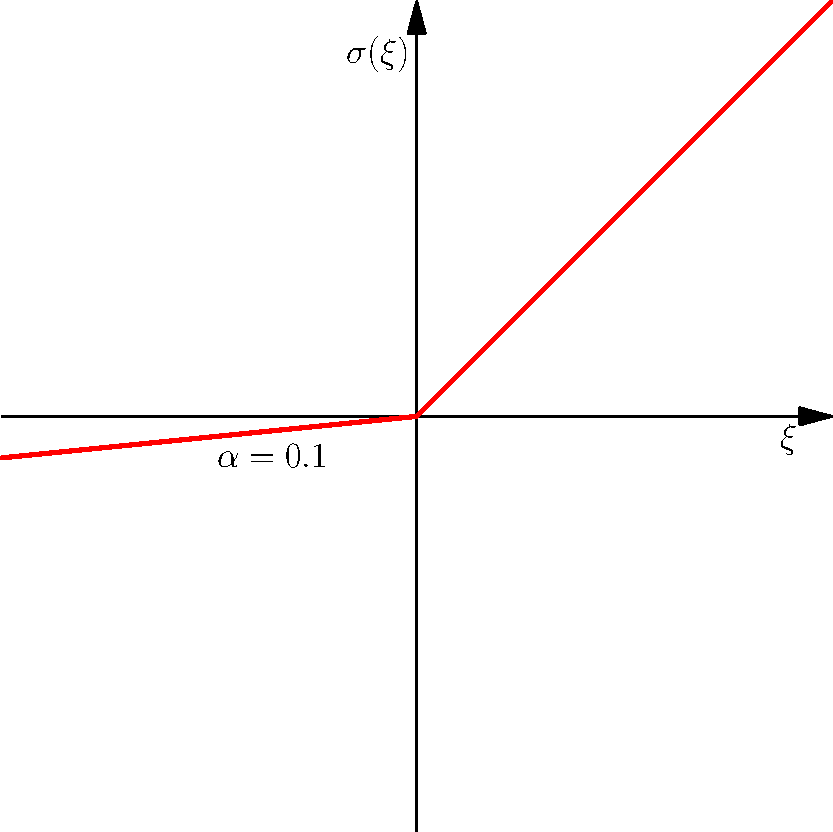
\includegraphics[width=0.25\textwidth]{fig/nn/lrelu.pdf}}\\
    \subfigure[Logistic]{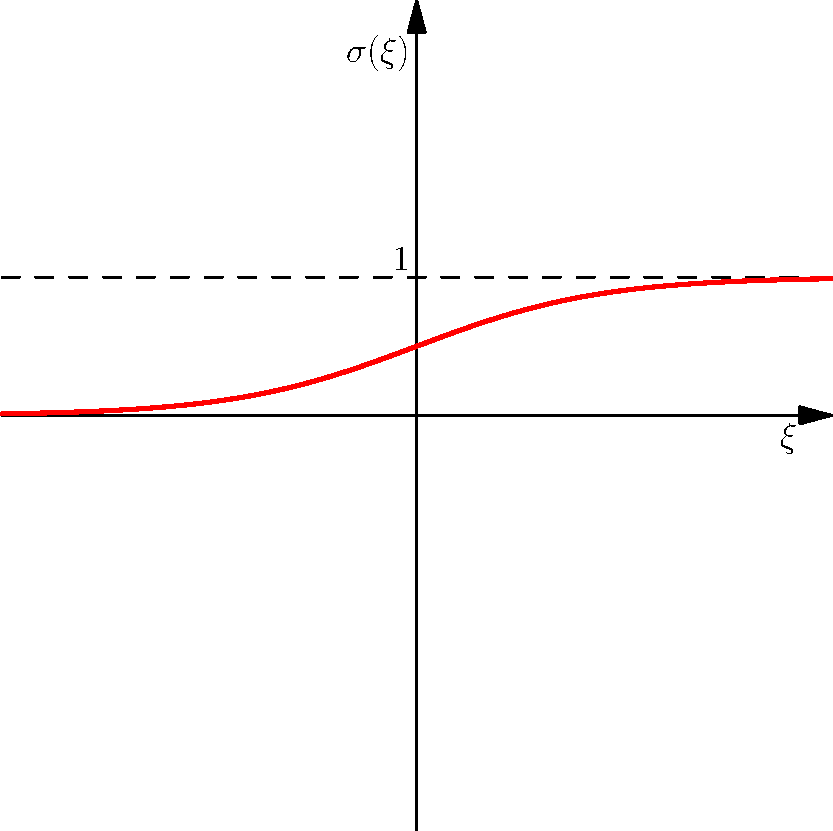
\includegraphics[width=0.25\textwidth]{fig/nn/logistic.pdf}}
    \subfigure[Tanh]{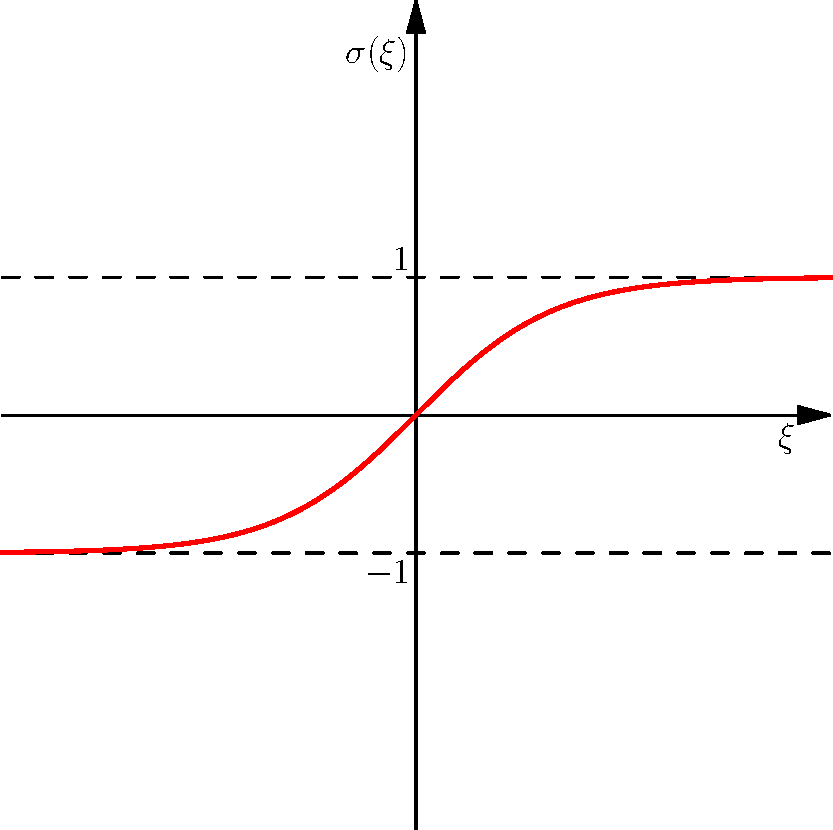
\includegraphics[width=0.25\textwidth]{fig/nn/tanh.pdf}}
    \subfigure[Sine]{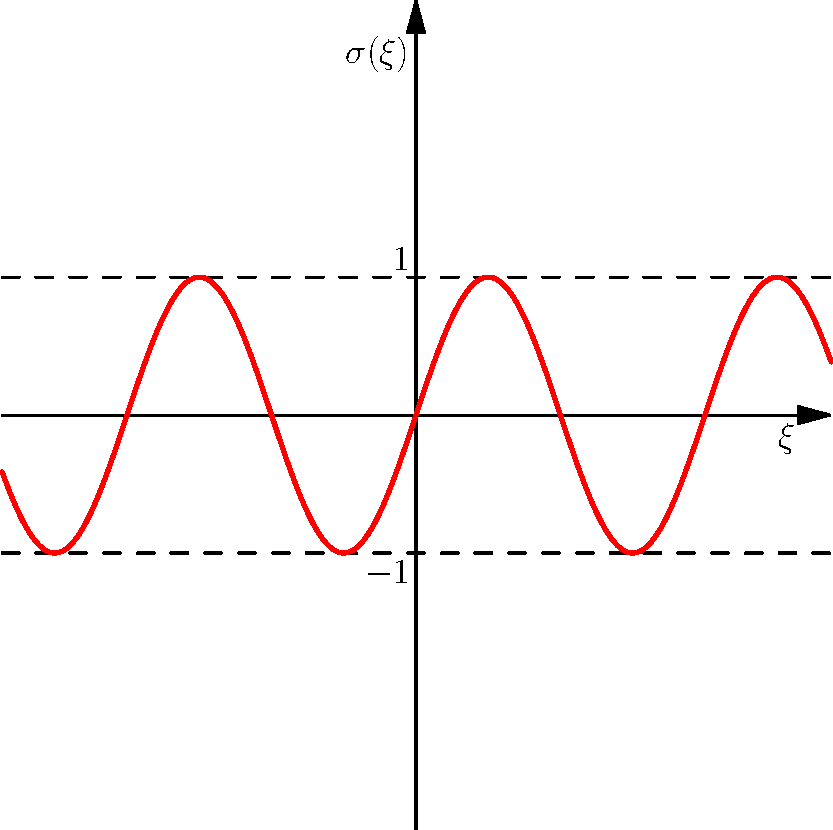
\includegraphics[width=0.25\textwidth]{fig/nn/sine.pdf}}
    \caption{Examples of activation functions}
    \label{fig:actfunc}
  \end{center}
\end{figure}

%\subsection*{Linear activation}
%The simplest activation corresponds to $\sigma(\xi) = \xi$. Some features of this function are
%\begin{itemize}
%  \item The function is infinitely smooth, but all derivatives beyond the second derivative are zero.
%  \item The range of the function is $(-\infty,\infty)$.
%  \item %In the absence of an output function $O$, 
%    Using the linear activation function (in all layers) will reduce the entire network to a single affine transformation of the input $\vx$. In other words, the network will be nothing more that a linear approximation of the target function $\vf$, which is not useful if $\vf$ is highly non-linear. 
%\end{itemize}
%
%\subsection*{Rectified linear unit (ReLU)}
%
%This function is piecewise linear and defined as
%\begin{equation}
%  \sigma(\xi) = \max\{0,\xi\} = \begin{cases} \xi, & \quad \text{if } \xi \geqslant 0 \\ 0, & \quad \text{if } \xi < 0  \end{cases}
%\end{equation}
%This is one of the most popular activation functions used in practice. Some features of this function are:
%\begin{itemize}
%  \item The function is continuous, while its derivative will be piecewise constant with a jump  $\xi = 0$. The second derivative will be a dirac function concentrated at $\xi=0$. In other words, the higher-order derivates (greater than 1) are not well-defined.
%  \item The range of the function is $[0,\infty)$.
%\end{itemize}
%
%\subsection*{Leaky ReLU}
%The ReLU activation leads to a null output from a neuron if the affine transformation of the neuron is negative. This can lead to the phenomena of \textbf{dying neurons} \cite{Mass2013} while training a neural network, where neurons drops out completely from the network and no longer contribute to the final prediction. To overcome this challenge, a leaky version ReLU was designed
%\begin{equation}
%  \sigma(\xi; \alpha) = \begin{cases} \xi, & \quad \text{if } \xi \geqslant 0 \\ \alpha \xi, & \quad \text{if } \xi < 0 \end{cases}
%\end{equation}
%where $\alpha$ becomes a network \textbf{hyper-parameter}. Some features of this function are:
%\begin{itemize}
%  \item The derivates of Leaky ReLU behave in the same way as those for ReLU.
%  \item The range of the function is $(-\infty,\,\infty)$.
%\end{itemize}
%
%\subsection*{Logistic function}
%The Logistic or Sigmoid activation function is given by
%\begin{equation}
%  \sigma(\xi) = \frac{1}{1 + e^{-\xi}}
%\end{equation}
%and has the following properties
%\begin{itemize}
%  \item The function is infinitely smooth and monotonic.
%  \item The range of the function is $(0,1)$, i.e., the function is bounded. Such a function is useful in representing probabilities. 
%  \item Since the derivative quickly decays to zero away from $\xi=0$, this activation function can lead to slow convergence of the network while training.
%\end{itemize}
%
%\subsection*{Tanh}
%The tanh function is can be seen as a symmetric extension of the logistic function
%\begin{equation}
%  \sigma(\xi) = \frac{e^{\xi} - e^{-\xi}}{e^{\xi} + e^{-\xi}}
%\end{equation}
%and has the following properties
%\begin{itemize}
%  \item The function is infinitely smooth and monotonic.
%  \item The range of the function is $(-1,1)$, i.e., the function is bounded. Note that it maps zeros input to zero, while pushing positive (negative) inputs to +1 (-1).
%  \item Similar to the logistic function, the derivative of tanh quickly decays to zero away from $\xi=0$ and can thus lead to slow convergence while training networks.
%\end{itemize}
%
%\subsection*{Sine}
%Recently, the sine function, i.e., $\sigma(\xi) = \sin(\xi)$ has been proposed as an efficient activation function \cite{Siren2020}. It has the best features of all the activation function discussed above:
%\begin{itemize}
%  \item The function is infinitely smooth.
%  \item The range of the function is $(-1,1)$, i.e., the function is bounded. 
%  \item None of the derivatives of this function decay to zero.
%\end{itemize}
%
%\begin{question}	
%  Can you think of an MLP architecture with the sine activation function, which leads to an approximation very similar to a Fourier series expansion?
%\end{question}

%\section*{Expressivity of a network}
%Let us try to understand the effects of $N_\theta$ increases. To see this, let us consider a simple example using the ReLU activation function, i.e., $\sigma(\xi) = \max\{\xi,0\}$. We set $d=D=1$, $L=1$ and the parameters
%\begin{align*}
%\vW^{(1)} = \begin{bmatrix} 2 \\ 1\end{bmatrix}, \quad \vb^{(1)} = \begin{bmatrix} -2 \\ 0 \end{bmatrix}, \quad \vW^{(2)} = \begin{bmatrix} 1 &  1 \end{bmatrix}, \quad b^{(2)} =  0.
%\end{align*}
%as shown in Figure \ref{fig:exp_eg}(a). Then the various layer outputs are 
%\begin{align*}
%x_1^{(1)} = \max\{2 x^{(0)}_1 - 2,0\},  \quad x_2^{(1)} = \max\{x^{(0)}_1,0\},  \quad x_1^{(2)} = \max\{2 x^{(0)}_1 - 2,0\} + \max\{x^{(0)}_1,0\}.
%\end{align*}
%Notice that while the the output $\vx^{(1)}$ of the hidden layer (see Figures \ref{fig:exp_eg}(b) and (c)) have only one corner/kink, the final output ends up having two kinks (see Figures \ref{fig:exp_eg}(d)).
%
%\begin{figure}[htbp!]
%  \begin{center}
%    \subfigure[MLP with $L=1$,$W=2$]{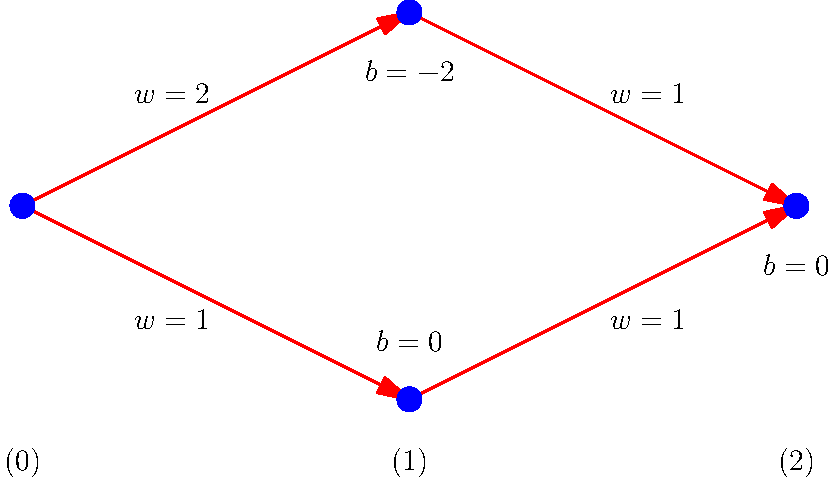
\includegraphics[width=0.45\textwidth]{fig/nn/expressivity_example_plot1.pdf}}
%    \subfigure[$x^{(1)}_1$ vs $x^{(0)}_1$]{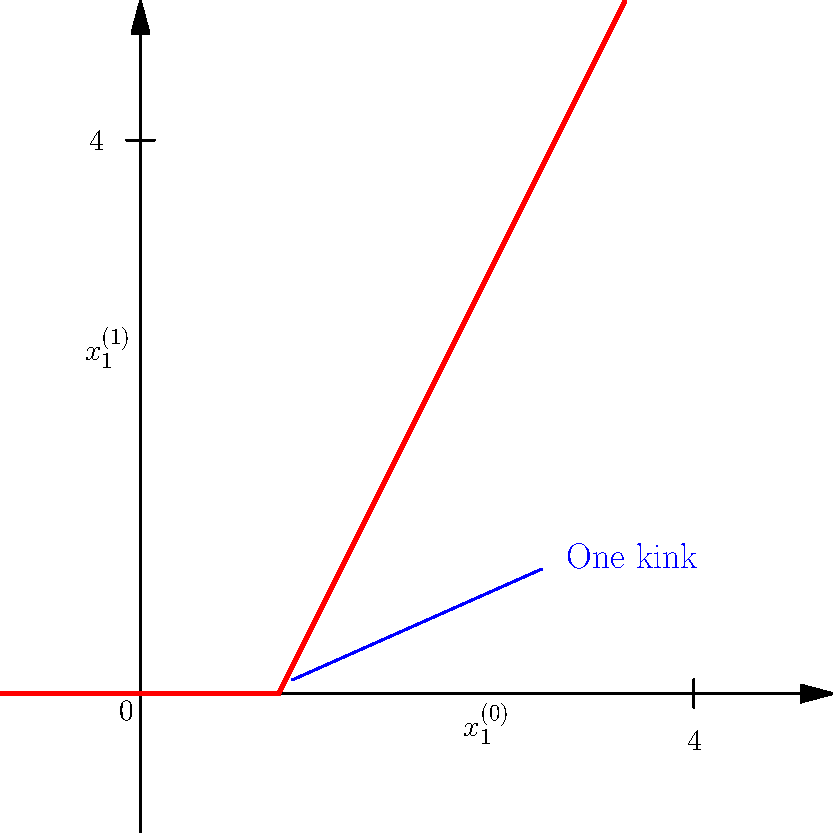
\includegraphics[width=0.45\textwidth]{fig/nn/expressivity_example_plot2.pdf}}
%    \subfigure[$x^{(1)}_2$ vs $x^{(0)}_1$]{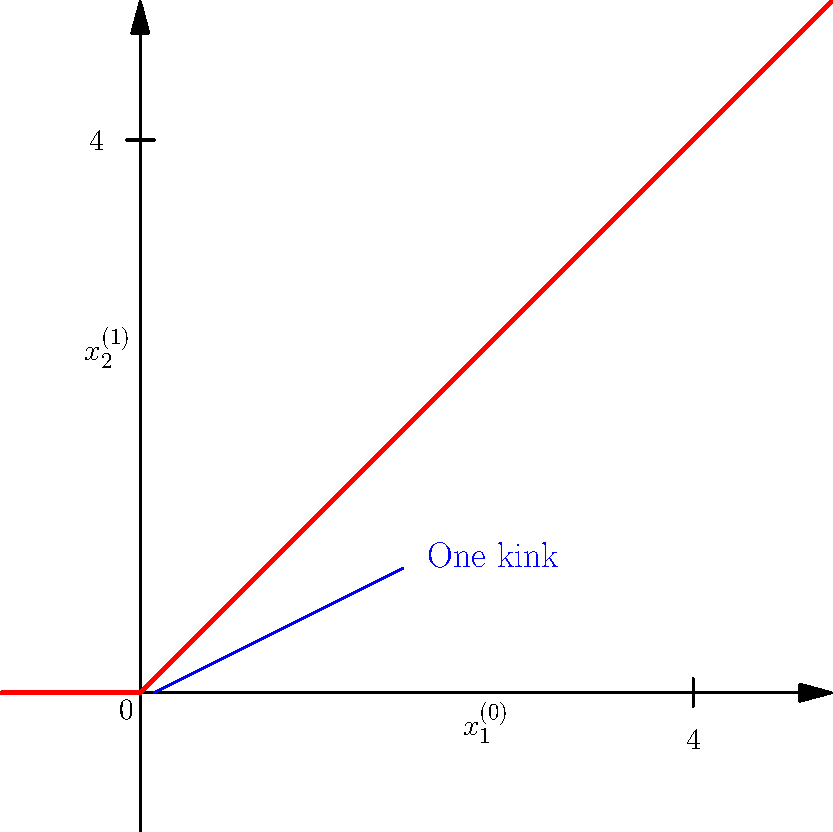
\includegraphics[width=0.45\textwidth]{fig/nn/expressivity_example_plot3.pdf}}
%    \subfigure[$x^{(2)}_1$ vs $x^{(0)}_1$]{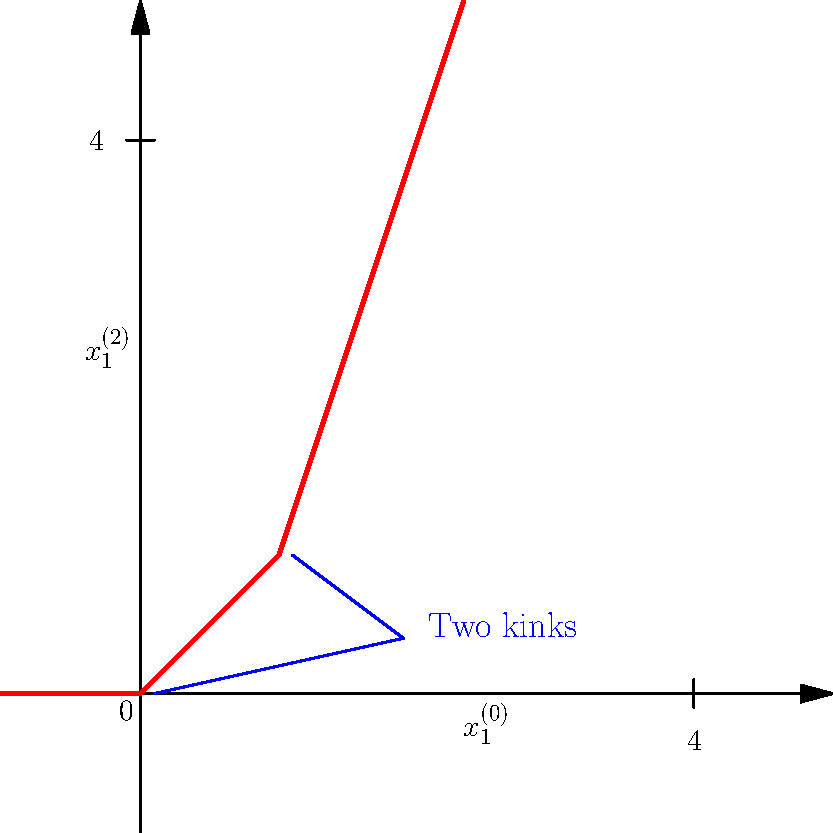
\includegraphics[width=0.45\textwidth]{fig/nn/expressivity_example_plot4.pdf}}
%    \caption{Examples to understand the expressivity of neural networks}
%    \label{fig:exp_eg}
%  \end{center}
%\end{figure}
%
%We generalize this formulation to a bigger network with $L$ hidden layers each of width $H$. Then one can expect that $x^{(1)}_i$, $1\leqslant i \leqslant H$ will have a single kink, with the location and angle of the kink depending on the weights and bias associated with each neuron of the hidden layer. The vector $\vx^{(1)}$ is passed to the next hidden layer, where each neuron will combine the single kinks and give an output with possibly $H$ kinks. Once again, the location and angles of the $H$ kinks in the output from each neuron of the second hidden layer will be different. The location of the kinks will be different because each neuron is allowed a different bias, and therefore can induce a different shift. Continuing this argument, one can expect the number of kinks to increase as $H$, $H^2$, $H^3$ as it passes through the various hidden layers with width $H$. In general the total number of kinks can grow as $H^L$. In other words, the networks have the ability to become more expressive as the depth (and width) of the network is increased.
%
\section*{Universal approximation results}\label{sec:uni_app_thms}
%To quantify the expressivity of networks in a mathematically rigorous manner, we look at some results about the approximation properties of MLPs. For these results, we assume $K \subset \Ro^d$ is a closed and bounded set.
Assume $K \subset \Ro^d$ is closed and bounded.

\begin{theorem}[\cite{Pinkus1999}]
Let $f:K\to\Ro$, i.e., $D=1$, be a continuous function. Then given an $\epsilon > 0$, there exists an MLP with a single hidden layer ($L=1$), arbitrary width $H$ and a non-polynomial continuous activation $\sigma$ such that
\begin{align*}
  \max_{\vx \in K} |\mathcal{F}(\vx;\btheta) - f(\vx)| \leqslant \epsilon.
\end{align*} 
\end{theorem}

\begin{theorem}[\cite{Kidger2020}]
Let $\vf:K \to \Ro^D$ be a continuous vector-valued function. Then given an $\epsilon >0$, there exists an MLP with arbitrary number of hidden layers $L$, each having width $H \geqslant d + D + 2$, a continuous activation $\sigma$ (with some additional mild conditions), such that
\begin{align*}
\max_{\vx \in K}  \|\mathcal{F}(\vx;\btheta) - \vf(\vx)\| \leqslant \epsilon.
\end{align*} 
\end{theorem}

\begin{theorem}[\cite{Yarotsky2021}]
Let $f:K \to \Ro$ be a function with two continuous derivates, i.e., $f \in C^2(K)$. Consider an MLP with ReLU activations and $H \geqslant 2d + 10$. Then there exists a network with this configuration such that the error converges as
\begin{align*}
\max_{\vx \in K}  |\mathcal{F}(\vx;\btheta) - \vf(\vx)| \leqslant C(N_\theta)^{-4}
\end{align*} 
where $C$ is a constant depending on the number of network parameters.
\end{theorem}

\newpage

%Numerical results like those mentioned above help demystify the ``black-box'' nature of neural network, and serve as useful practical guidelines when designing network architectures.

\section*{Training, Validation and Testing of NN}
%Now that we have a better understanding of the architecture of MLPs, we would now like to discuss how the parameters of these networks are set to approximate some target function. We restrict our discussions to the framework of supervised learning.

Let us assume that we are given a dataset of pairwise samples $\mathcal{S} = \{(\vx_i,\vy_i): 1 \leqslant i \leqslant N\}$ corresponding to a target function $\vf: \vx\to\vy$. We wish to approximate this function using the neural network $\ds\mathcal{F}(\vx; \btheta, \Hp)$
where $\btheta$ are the network parameters defined before, while $\Hp$ corresponds to the \textbf{hyper-parameters} of the network such as the depth $L+1$, width $H$, type of activation function $\sigma$, etc. The strategy to design a robust network involves three steps:
\begin{enumerate}
\item Find the optimal values of $\btheta$ (for a fixed $\Hp$)  in the \textbf{training} phase.
\item Find the optimal values of $\Hp$ in the \textbf{validation} phase.
\item Test the performance of the network on unseen data on the \textbf{testing} phase.
\end{enumerate}

To accomplish these three tasks, it is first customary to split the dataset $\mathcal{S}$ into three distinct parts: a \textbf{training set} with $N_{\text{train}}$ samples, a \textbf{validation set} with $N_{\text{val}}$ samples and \textbf{test set} with $N_{\text{test}}$ samples, with $N = N_{\text{train}} + N_{\text{val}} + N_{\text{test}}$. Typically, one uses around 60\% of the samples as training samples, 20\% as validation samples and the remaining 20\% for testing. 

Splitting the dataset is necessary as neural networks are heavily over-parameterized functions. The large number of degrees of freedom available to model the data can lead to over-fitting the data. This happens when the error or noise present in the data drives the behavior of the network more than the underlying input-output relation itself. Thus, a part of the data is used to determine $\btheta$, and another part to determine the hyper-parameters $\Hp$. The remainder of the data is kept aside for testing the performance 
 of the trained network on unseen data, i.e., the network's ability to \textbf{generalize} well.

Now let us discuss how this split is used during the three phases in further details:

\paragraph{Training:}
Training the network makes use of the training set $\mathcal{S}_{\text{train}}$ to find $\ds\btheta^* = \amin_{\btheta} \Pi_\text{train}(\btheta)$ where
\begin{align*}
  \Pi_\text{train} (\btheta)= \frac{1}{N_\text{train}} \sum_{\substack{i=1\\(\vx_i,\vy_i) \in \mathcal{S}_{\text{train}}}}^{N_\text{train}} \|\vy_i - \mathcal{F}(\vx_i; \btheta, \Hp)\|^2
\end{align*}
for some fixed $\Hp$. The optimal $\btheta^*$ is obtained using a suitable gradient based algorithm (will be discussed later). The function $\Pi_\text{train}$ is referred to as the loss function. In the example above we have used the mean-squared loss function. Later we will consider other types of loss functions. 

\paragraph{Validation:}
Validation of the network involves using the validation set $\mathcal{S}_{\text{val}}$ to find $\ds\Hp^* = \amin_{\Hp} \Pi_\text{val}(\Hp)$ where
\begin{align*}
  \Pi_\text{val} (\Hp)= \frac{1}{N_\text{val}} \sum_{\substack{i=1\\(\vx_i,\vy_i) \in \mathcal{S}_{\text{val}}}}^{N_\text{val}} \|\vy_i - \mathcal{F}(\vx_i; \btheta^*, \Hp)\|^2
\end{align*}
The optimal $\Hp^*$ is obtained using a techniques such as (random or tensor) grid search.

\paragraph{Testing:} Once the "best" network is obtained, characterized by $\btheta^*$ and $\Hp^*$, it is evaluated on the test set $\mathcal{S}_\text{test}$ to estimate the networks performance on data not used during the first two phases. 
\begin{align*}
  \Pi_\text{test} = \frac{1}{N_\text{test}} \sum_{\substack{i=1\\(\vx_i,\vy_i) \in \mathcal{S}_{\text{test}}}}^{N_\text{test}} \|\vy_i - \mathcal{F}(\vx_i; \btheta^*, \Hp^*)\|^2.
\end{align*}
This testing error is also known as the (approximate) \textbf{generalizing error} of the network.

\begin{example}
  Let us consider an MLP where all hyper-parameters are fixed except for the following flexible choices: $\ds\sigma \in \{\text{ReLU, tanh}\}, \quad L \in \{10,\,20\}$. We use the following algorithm
\begin{enumerate}
  \item For each possible $\sigma$, $L$ pair:
    \begin{enumerate}
      \item Find $\btheta^* = \amin_{\btheta} \Pi_\text{train}(\btheta)$
      \item With this $\btheta^*$, evaluate $\Pi_\text{val}(\Hp)$
    \end{enumerate}
  \item Select $\Hp^*$ to be the one that gave the smallest value of $\Pi_\text{val}(\Hp)$.	
  \item Finally, report $\Pi_\text{test}$ for this $\Hp^*$ and the corresponding $\btheta^*$.
\end{enumerate}
\end{example}

\section*{Generalizability} 
If we train a network that has a small value of $\Pi_\text{train}$ and $\Pi_\text{val}$, does it ensure that $\Pi_\text{test}$ will be small? This question is addressed by studying the \textbf{generalizability} of the trained network, i.e., it capability to perform well on data not seen while training/validating the network. If the network is trained to overfit the training data, the network will typically lead to poor predictions on test data. Typically, if $\mathcal{S}_\text{train}$, $\mathcal{S}_\text{val}$ and $\mathcal{S}_\text{test}$ are chosen from the same distribution of data, then a small value of $\Pi_\text{train},\Pi_\text{val}$ can lead to small values of $\Pi_\text{test}$. Let us look at the commonly used technique to avoid data overfitting, called \textbf{regularization}.

\subsection*{Regularization}\label{sec:reg}
Neural networks are almost always \textbf{over-parametrized}, i.e., $N_\theta \gg N$ where $N$ is the number of training samples. This would lead to a highly non-linear network model, for which the loss function $\Pi(\btheta)$ (where we omit the subscript "train" for brevity) can have a landscape with many local minimas (see Figure \ref{fig:reg}(a)). Then how do we determine which minima leads to a better generalization? To nudge the choice of $\btheta^*$ in a more favorable direction, a regularization technique can be employed.

\begin{figure}[htbp!]
\begin{center}
\subfigure[Loss function landscape]{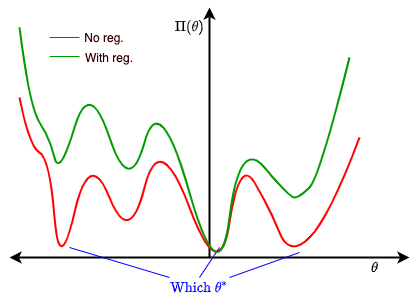
\includegraphics[width=0.4\textwidth]{fig/nn/reg1a.png}}
\subfigure[Network sensitivity]{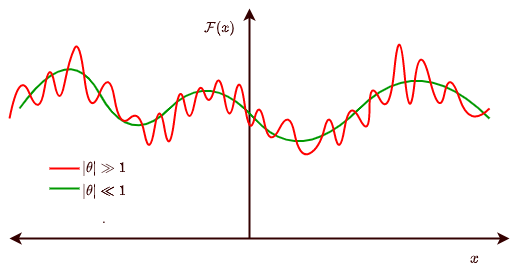
\includegraphics[width=0.55\textwidth]{fig/nn/reg1b.png}}
\caption{The effect of regularization on the loss function. We have assumed a scalar $\theta$ for easier illustration.}
\label{fig:reg}
\end{center}
\end{figure}

The simplest method of regularization involves augmenting a penalty term to the loss function:
\begin{align*}
  \Pi(\btheta) \longrightarrow \Pi(\btheta) + \alpha\,\|\btheta\|, \quad \alpha \geqslant 0
\end{align*}
where $\alpha$ is a regularization hyper-parameter, and $\|\btheta\|$ is a suitable norm of the network parameters $\btheta$. This augmentation can change the landscape of $\Pi(\btheta)$ as illustrated in Figure \ref{fig:reg}(a). In other words, such a regularization encourages the selection of a minima corresponding to smaller values of the parameters $\btheta$. 

It is not obvious why a smaller value of $\btheta$ would be a better choice. To see why this is better, consider the intermediate network output
\begin{align*}
  x_1^{(1)} = \sigma\big(W_{1j}^{(1)} x_j^{(0)} + b^{(1)}_1\big),
\end{align*}
which gives
\begin{align*}
\df{x_1^{(1)}}{x_1^{(0)}} = \sigma^\prime\big(W_{1j}^{(1)} x_j^{(0)} + b^{(1)}_1\big) W_{11}^{(1)}  \propto W_{11}^{(1)}.
\end{align*}
Since this derivate scales with $W_{11}^{(1)}$, this implies that $\Big|\df{\mathcal{F}(\vx)}{x_1^{(0)}}\Big|$ scales with $W_{11}^{(1)}$ as well. If $\ds|W_{11}^{(1)}|\gg 1$, then network would be very sensitive to even small changes in the input $x_1^{(0)}$, i.e., the network would be ill-posed. As illustrated in Figure \ref{fig:reg}(b), using a proper regularization would help avoid over fitting.

Let us consider some common types of regularization:
\begin{itemize}
\item \textbf{$l_2$ regularization}: Here we use the $l_2$ norm in the regularization term
\begin{align*}
\| \btheta \| = \|\btheta\|_2 = \left(\sum_{i=1}^{N_\theta} \theta_i^2\right)^{1/2}.
\end{align*}	
\item \textbf{$l_1$ regularization}: Here we use the $l_1$ norm in the regularization term
\begin{align*}
\| \btheta \| = \|\btheta\|_1 = \sum_{i=1}^{N_\theta} |\theta_i|,
\end{align*}
which promotes the sparsity of $\btheta$.
\end{itemize}

\section*{Gradient descent}
Recall that we wish to solve the minimization problem $\btheta^* = \amin \Pi(\btheta)$ in the training phase. This minimization problem can be solved using gradient descent (GD), also known as steepest descent. Consider the Taylor expansion about $\btheta_0$
\begin{align*}
  \Pi(\btheta_0 + \Delta \btheta) = \Pi(\btheta_0) + \df{\Pi}{\btheta}(\btheta_0) \cdot \Delta \btheta + \df{^2\Pi}{\theta_i\partial\theta_j}(\widehat{\btheta}) \Delta \theta_i \Delta \theta_j
\end{align*}
for some $\widehat{\btheta}$ in a small neighbourhood of $\btheta_0$. When $|\Delta \btheta |$ is small and assuming $\df{^2\Pi}{\theta_i\partial\theta_j}$ is bounded, we can neglect the second order term and just consider the approximation
\begin{align*}
\Pi(\btheta_0 + \Delta \btheta) \approx \Pi(\btheta_0) + \df{\Pi}{\btheta}(\btheta_0) \cdot \Delta \btheta. 
\end{align*}
In order to lower the value of the loss function as much as possible compared to its evaluation at $\btheta_0$, i.e. minimize $\Delta \Pi = \Pi(\btheta_0 + \Delta \btheta) - \Pi(\btheta_0)$, we need to choose the step $\Delta\btheta$ in the opposite direction of the gradient, i.e.:
\begin{align*}
  \Delta \btheta = - \eta\,\df{\Pi}{\btheta}(\btheta_0)
\end{align*}
with the step-size $\eta \geqslant 0$, also known as the \textbf{learning-rate}. This is yet another hyper-parameter that we need to tune during the validation phase. This is the crux of the GD algorithm, and can be summarized as follows:
\begin{enumerate}
  \item Initialize $k=0$ and $\btheta_0$
  \item While $|\Pi(\btheta_k)| > \epsilon_1$, do
    \begin{enumerate}
      \item Evaluate $\df{\Pi}{\btheta}(\btheta_k)$
      \item Update $\btheta_{k+1} = \btheta_k - \eta\,\df{\Pi}{\btheta}(\btheta_k)$
      \item Increment $k = k + 1$
    \end{enumerate}
\end{enumerate}

\textbf{Convergence:} Assume that $\Pi(\btheta)$ is convex and differentiable, and its gradient is Lipschitz continuous with Lipschitz constant  $\mathcal{K}$. Then for a $\eta \leqslant 1/\mathcal{K}$ , the GD updates converges as
\begin{align*}
\|\btheta^* - \btheta_k\|_2 \leqslant \frac{C}{k}.
\end{align*}

However, in most scenarios $\Pi(\btheta)$ is not convex. If there is more than one minima, then what kind of minima does GD like to pick? To answer this, consider the loss function for a scalar $\theta$ as  shown in Figure \ref{fig:GD}, which has two valleys. Let's assume that the profile of $\Pi(\theta)$ in the each valley can be approximated by a (centered) parabola
\begin{align*}
\Pi(\theta) \approx \frac{1}{2} a \theta^2
\end{align*}
where $a > 0$ is the  curvature of each valley. Note that the curvature of the left valley is much smaller than the curvature of the right valley. Let's pick a constant learning rate $\eta$ and a starting value $\theta_0$ in either of the valleys. Then, 
\begin{align*}
\df{\Pi}{\theta}(\theta_0) = a \theta_0
\end{align*}
and the new point after a GD update will be $\theta_1 = \theta_0(1-a\eta)$. Similarly, it is easy to see that all subsequent iterates write $\theta_{k+1} = \theta_k(1-a\eta)$. For convergence, we need
\begin{align*}
\left| \frac{\theta_{k+1}}{\theta_k}\right| < 1 \quad \implies |1 - a \eta| < 1.
\end{align*}
Since $a>0$ in the valleys, we will need the following condition on the learning rate
\begin{align*}
-1 < 1 - a \eta \implies a\eta < 2.
\end{align*}
If we fix $\eta$, then for convergence we need the local curvature to satisfy $a < 2/\eta$. In other words, GD will prefer to converge to a minima with a flat/small curvature, i.e., it will prefer the minima in the left valley. If the starting point is in the right valley, there is a chance that we will keep overshooting the right minima and bounce off the opposite wall till the GD algorithm slingshots $\theta_k$ outside the valley. After this it will enter the left valley with a smaller curvature and gradually move towards its minima.

\begin{figure}[htbp!]
\begin{center}
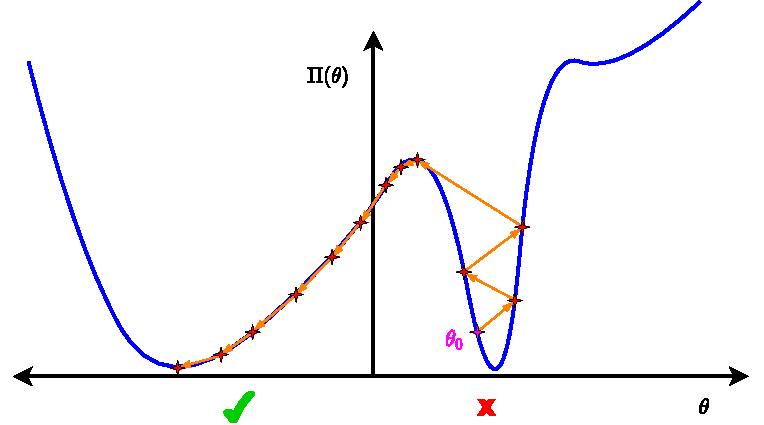
\includegraphics[width=0.5\textwidth]{fig/nn/GD.pdf}
\caption{GD prefers flatter minimas.}
\label{fig:GD}
\end{center}
\end{figure}

While it is clear that GD prefers flat minima, what is not clear is why are flat minima better. There is empirical evidence that the parameter values obtained at flat minima tend to generalize better, and therefore are to be preferred. 

\section*{Some advanced optimization algorithms}
We discussed how GD can be used to solve the optimization problem involved in training neural networks. Let us look at a few advanced and popular optimization techniques motivated by GD. 

In general, the update formula for most optimization algorithms make use of the following formula
\begin{equation}
[\btheta_{k+1}]_i = [\btheta_{k}]_i - [\eta_k ]_i [\vg_k]_i, \quad 1 \leqslant i \leqslant N_\theta,
\end{equation}
where $[\eta_k]_i$ is the component-wise learning rate and the vector-valued function $\g$ depends/approximates the gradient. Note that the notation $[.]_i$ is used to denote the $i$-th component of the vector. Also note that the learning rate is allowed to depend on the iteration number $k$. The GD method makes use of 
\begin{align*}
[\eta_k ]_i = \eta, \quad \g_k = \df{\Pi}{\btheta}(\btheta_k).
\end{align*}
An issue with the GD method is that the convergence to the minima can be quite slow if $\eta$ is not suitably chosen. For instance, consider the objective function landscape shown in Figure \ref{fig:gd_zigzag}, which has sharper gradients along the $[\theta]_2$ direction compared to the $[\theta]_1$ direction. If we start from a point, such as the one shown in the figure, then if $\eta$ is too large (but still within the stable bounds) the updates will keep zig-zagging its way towards the minima. Ideally, for the particular situation shown in Figure \ref{fig:gd_zigzag}, we would like the steps to take longer strides along the $[\theta]_1$ compared to the $[\theta]_2$ direction, thus reaching the minima faster. 

\begin{figure}[htbp!]
\begin{center}
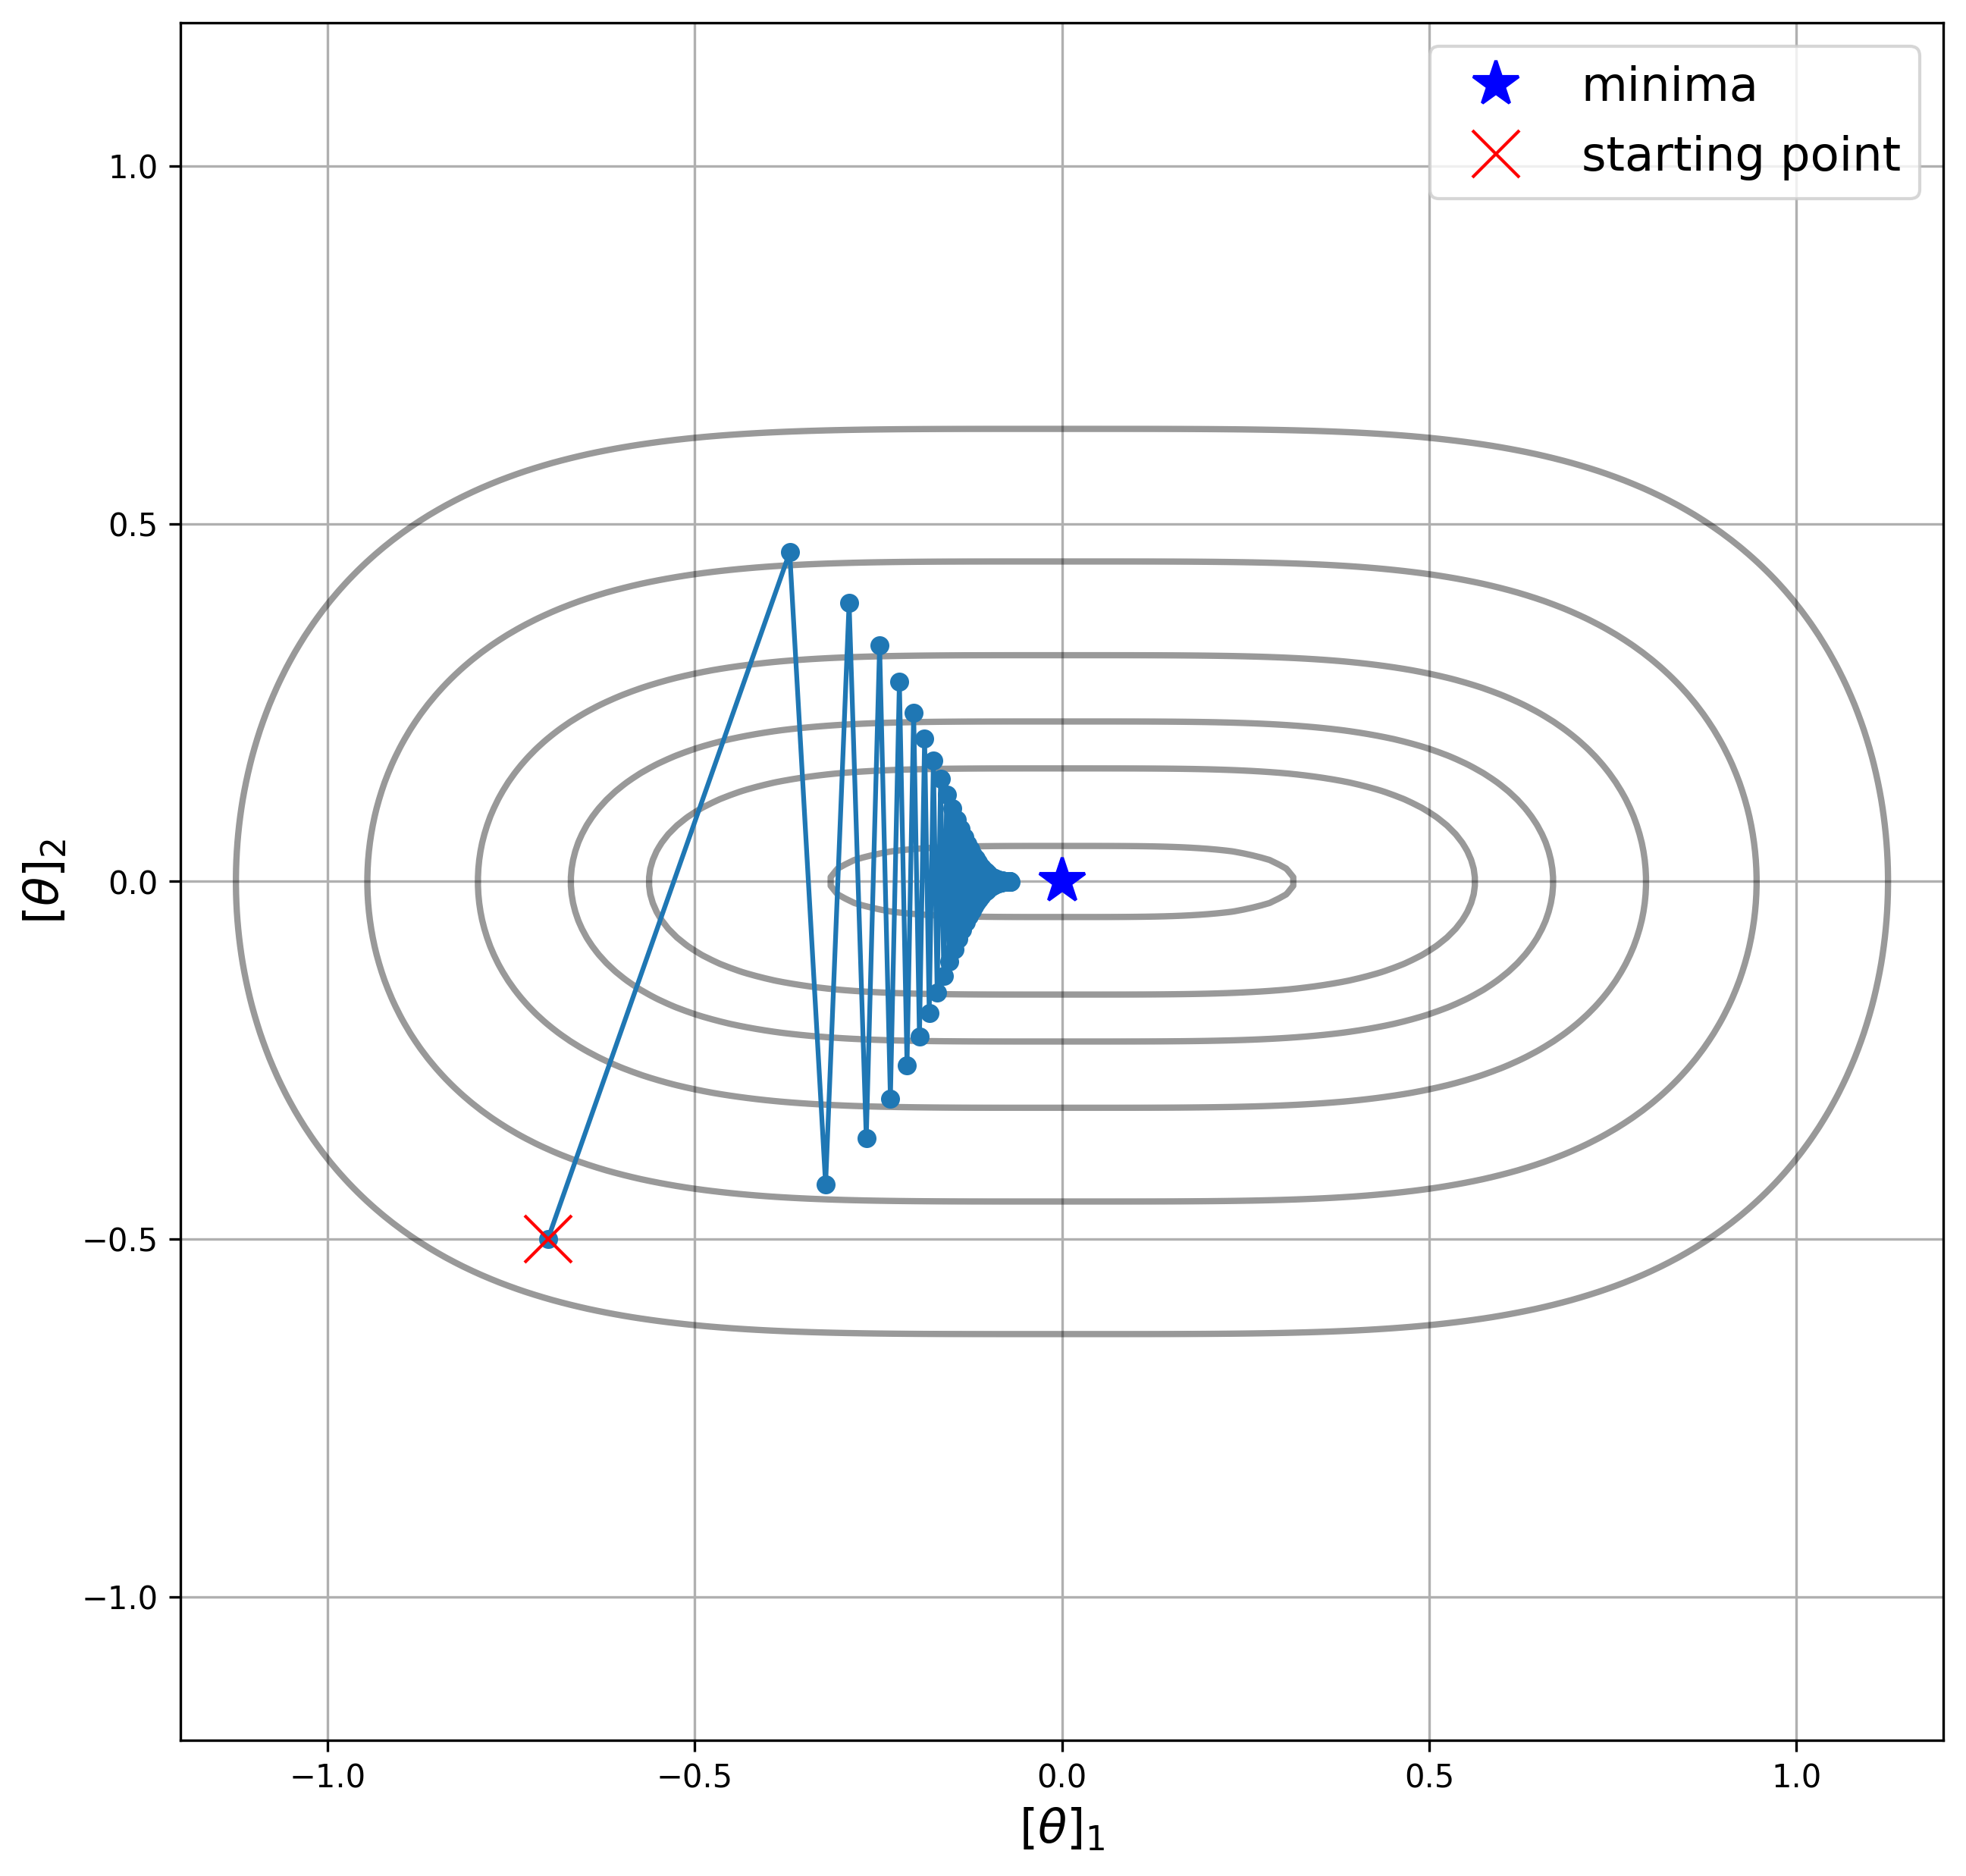
\includegraphics[width=0.5\textwidth]{fig/nn/gd_zigzag.png}
\caption{Zig-zagging updates with GD.}
\label{fig:gd_zigzag}
\end{center}
\end{figure}

Let us look at two popular methods that are able to overcome some of the issues faced by GD.

\subsection*{Momentum methods}
Momentum methods make use of the history of the gradient, instead of just the gradient at the previous step. The formula for the update is given by
\begin{align*}
[\eta_k ]_i = \eta, \quad \g_k = \beta_1 \g_{k-1} + (1-\beta_1) \df{\Pi}{\btheta}(\btheta_k), \quad \g_{-1} = 0
\end{align*}
where $\g_k$ is a weighted moving average of the gradient. This weighting is expected to smoothen out the zig-zagging seen in Figure \ref{fig:gd_zigzag} by cancelling out the components of gradient along the $[\theta]_2$ direction and move more smoothly towards the minima. A commonly used value for $\beta_1$ is 0.9. 

\subsection*{Adam}
The Adam optimization was introduced by Kingma and Ba \cite{kingma2017adam}, which makes use of the history of the gradient as well the second moment (which is a measure of the magnitude) of the gradient. For an initial learning rate $\eta$, the updates are given by
\begin{equation}
\begin{aligned}
\g_k &= \beta_1 \g_{k-1} +  (1-\beta_1) \df{\Pi}{\btheta}(\btheta_k) \\
[\G_k]_i &= \beta_2[\G_{k-1}]_i + (1-\beta_2) \left(\df{\Pi}{\btheta_i}(\btheta_k)\right)^2\\
[\eta_k ]_i &=\frac{\eta}{\sqrt{[\G_k]_i} + \epsilon} 
\end{aligned}
\end{equation}
where $\g_k$ and $\G_k$ are the weighted running averages of the gradients and the square of the gradients, respectively. The recommended values for the hyper-parameters are $\beta_1 = 0.9$, $\beta_2 = 0.999$ and $\epsilon=10^{-8}$. Note that the learning rate for each component is different. In particular, the larger the magnitude of the gradient for a component the smaller is its learning rate. Referring back to the example in Figure \ref{fig:gd_zigzag}, this would mean a smaller learning rate for $\theta_2$ in comparison to $\theta_1$, and therefore will help alleviate the zig-zag path of the optimization algorithm. 

\begin{remark}
The Adam algorithm also has additional correction steps for $\g_k$ and $\G_k$ to improve the efficiency of the algorithm. See \cite{kingma2017adam} for details.
\end{remark}


\subsection*{Stochastic optimization}
We note that the training loss can be rewritten as
\begin{align*}
\Pi(\btheta) = \frac{1}{N_\text{train}} \sum_{i=1}^{N_\text{train}} \Pi_i(\btheta), \quad \Pi_i(\btheta) = \|\vy_i - \mathcal{F}(\vx_i; \btheta, \Hp)\|^2
\end{align*}
Thus, the gradient of the loss function is
\begin{align*}
  \df{\Pi}{\btheta}(\btheta) = \frac{1}{N_\text{train}} \sum_{i=1}^{N_\text{train}}\df{\Pi_i}{\btheta}(\btheta)
\end{align*}
However, taking the summation of gradients can be very expensive since $N_\text{train}$ is typically very large, $N_\text{train} \sim 10^6$. One easy way to circumvent this problem is to use the following update formula (shown here for the GD method)
\begin{equation}\label{eqn:sgd}
  \btheta_{k+1} = \btheta_k - \eta_k\,\df{\Pi_i}{\btheta}(\btheta_k),
\end{equation}
where $i$ is randomly chosen for each update step $k$. This is known as  \textbf{stochastic gradient descent}. Remarkably, this modified algorithm does converge assuming that $\Pi_i(\btheta)$ is convex and differentiable, and $\eta_k \sim 1/\sqrt{k}$ (\cite{nemirovski90}). To illustrate why $\eta_k$ needs to decay, consider the toy function(s) for $\btheta \in \Ro^2$
\begin{equation}
  \begin{aligned}
    &\Pi_1(\btheta) = ([\theta]_1 - 1)^2 + ([\theta]_2 - 1)^2 \\
    &\Pi_2(\btheta) = ([\theta]_1 + 1)^2 + 0.5\,([\theta]_2 - 1)^2\\
    &\Pi_3(\btheta) = 0.7\,([\theta]_1 +1)^2 + 0.5\,([\theta]_2 +1)^2\\
    &\Pi_4(\btheta) = 0.7\,([\theta]_1 - 1)^2 + \frac{1}{2}\,([\theta]_2 + 1)^2\\
    &\Pi(\btheta) = \frac{1}{4} \big(\Pi_1(\btheta) + \Pi_2(\btheta) + \Pi_3(\btheta) + \Pi_4(\btheta)\big).
  \end{aligned}
\end{equation}
The contour plots of these functions in shown in Figure \ref{fig:sgd}(a), where the black contour plots corresponds to $\Pi(\btheta)$.  Note that the $\btheta^* = (0,0)$ is the unique minima for $\Pi(\btheta)$. We consider solving with the SGD algorithm with a constant learning rate $\eta_k=0.4$ and a decaying learning rate $\eta_k = 0.4/\sqrt{k}$. Starting with $\btheta_0=(-1.0,2.0)$ and randomly selecting $i \in {1,2,3,4}$ for each step $k$, we run the algorithm for 10,000 iterations. The first 10 steps with each learning rate is plotted in Figure \ref{fig:sgd}(a). We can clearly see that without any decay in the learning rate, the SGD algorithm keeps overshooting the minima. In fact, this behaviour continues for all future iterations as can be seen in Figure \ref{fig:sgd}(b) where the norm of the updates does not decay (we expect it to decay to $|\btheta^*| = 0$). On the other hand, we quickly move closer to $\btheta^*$ if the learning rate decays as $1/\sqrt{k}$. 

The reason for reducing the step size as we approach closer to the minima is that far away from the minima for $\Pi$ the gradient vector for $\Pi$ and all the individual $\Pi_i$'s align quite well. However, as we approach closer to the minima for $\Pi$ this is not the case and therefore one is required to take smaller steps so as not be thrown off to a region far away from the minima. 

\begin{figure}[htbp!]
  \begin{center}
    \subfigure[Function contours and paths]{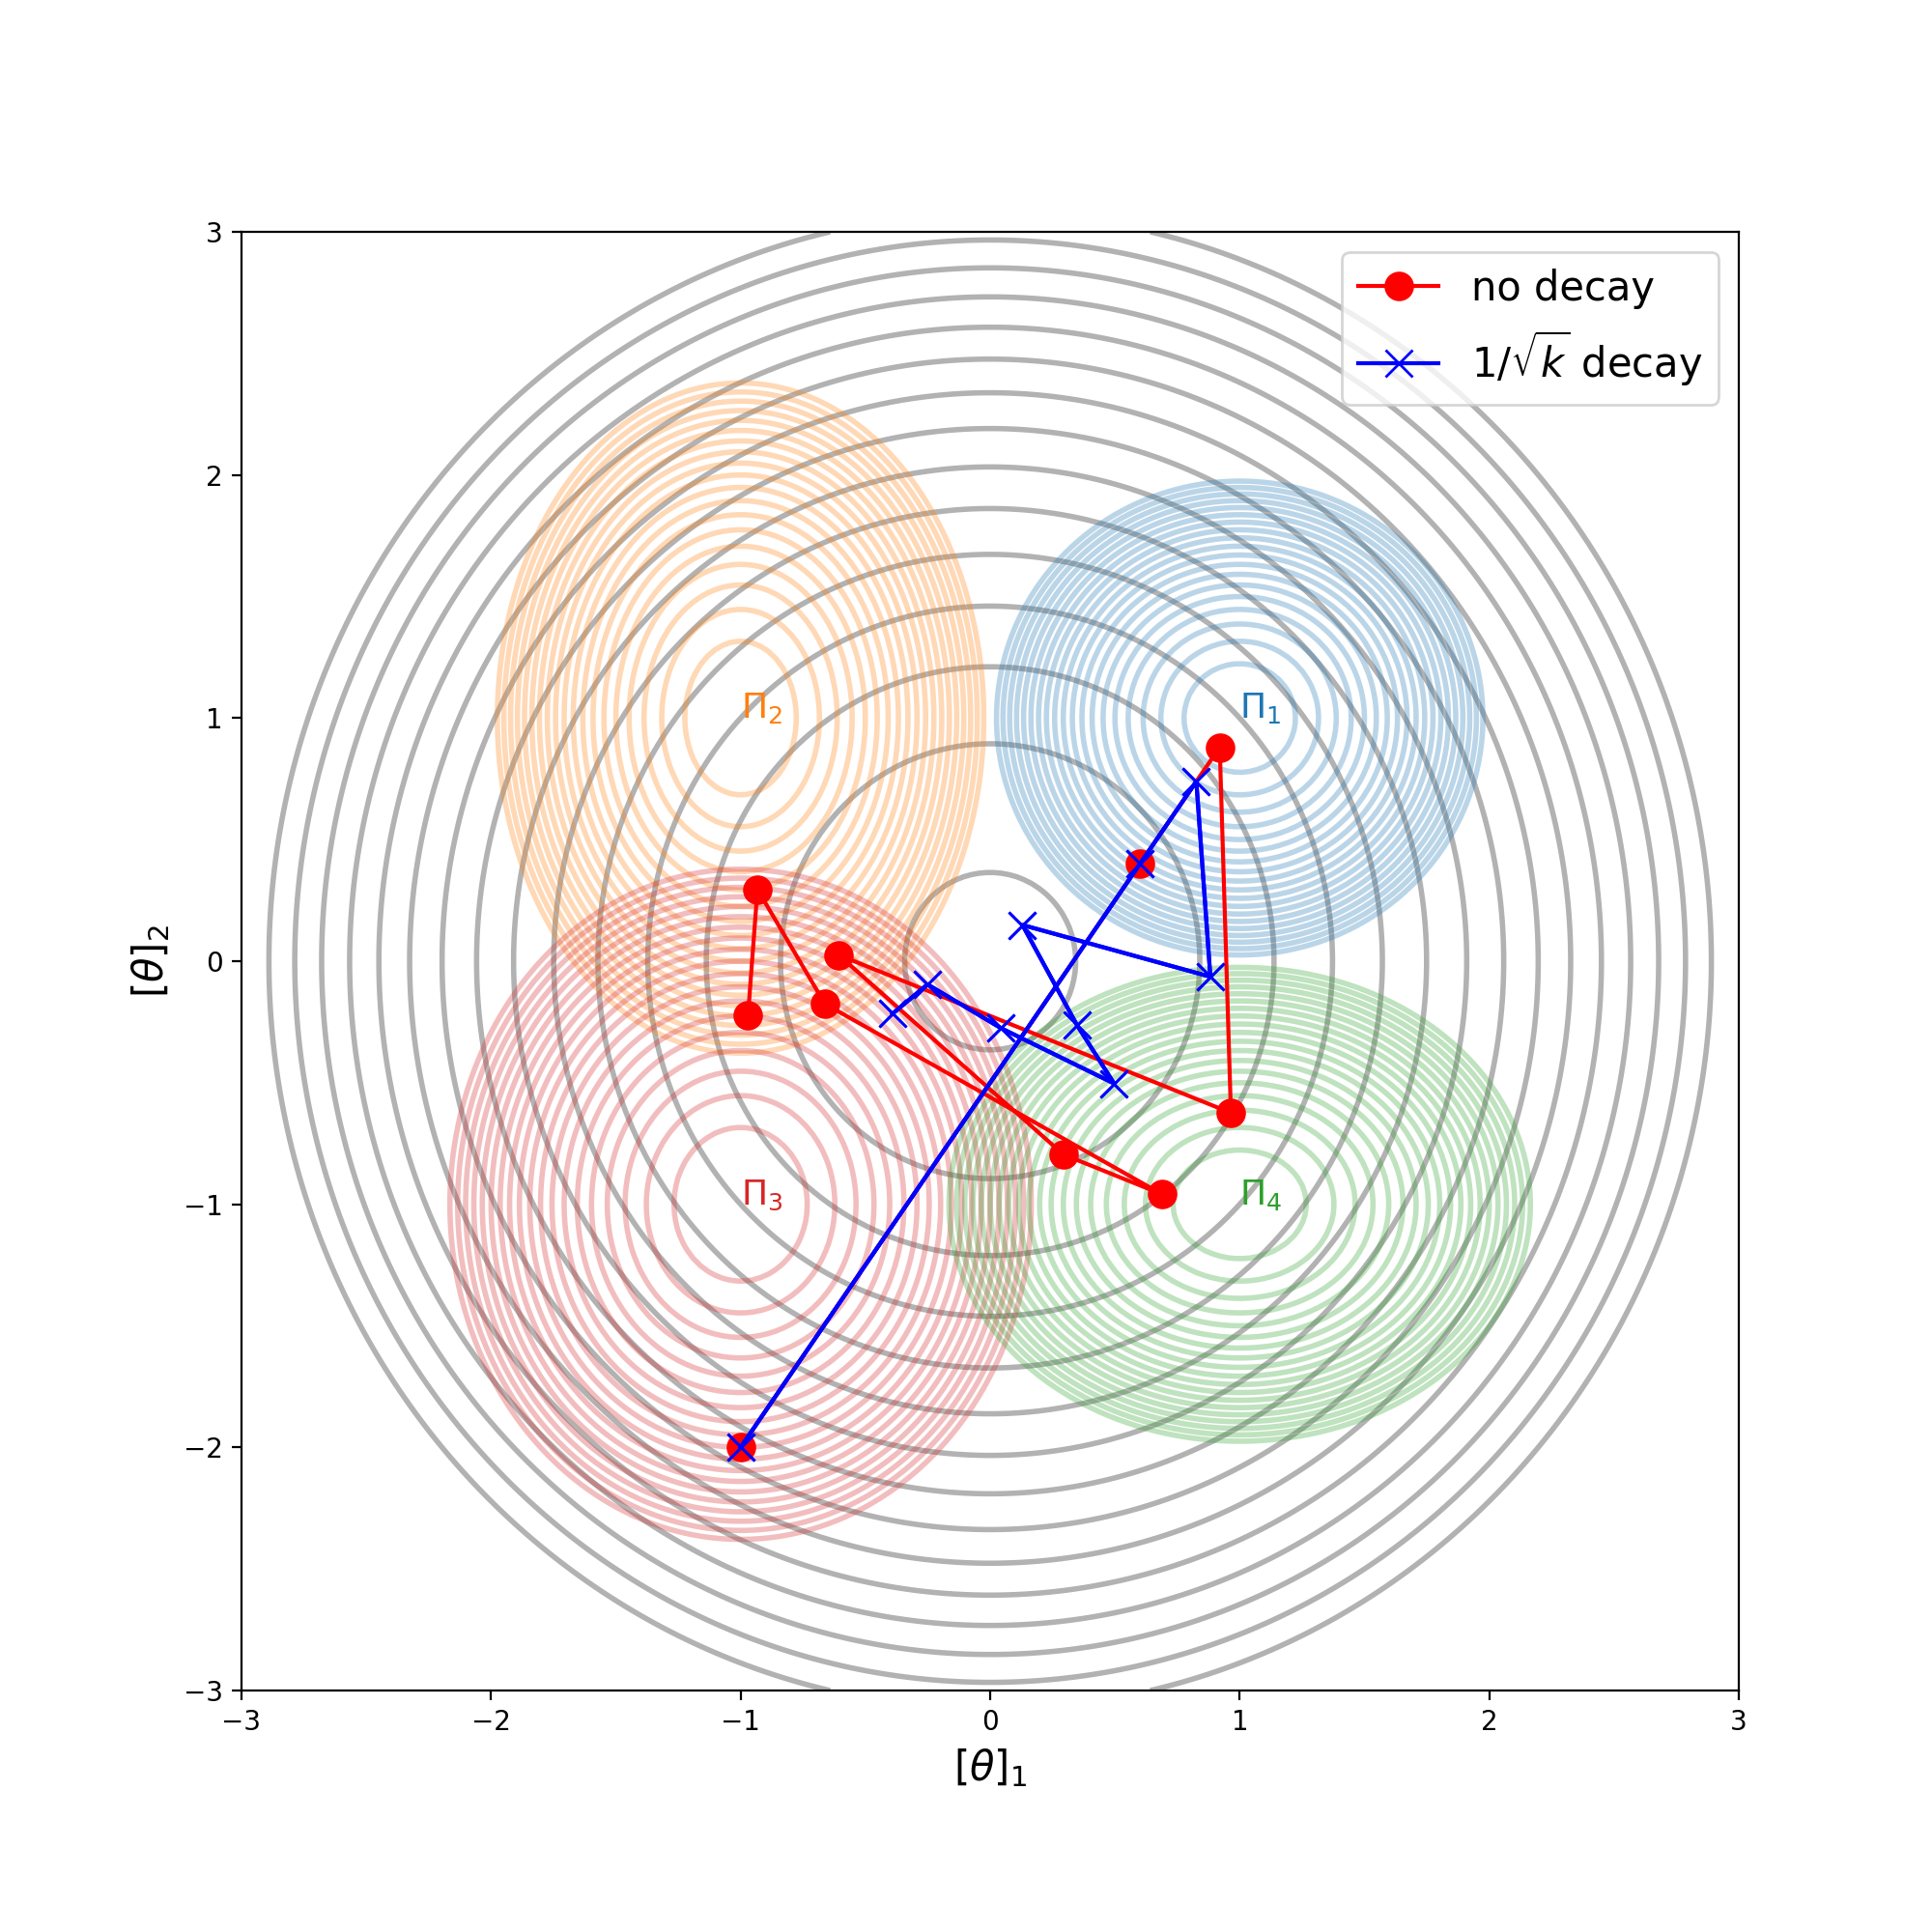
\includegraphics[width=0.45\textwidth]{fig/nn/contour_sgd.png}}
    \subfigure[Norm of updates]{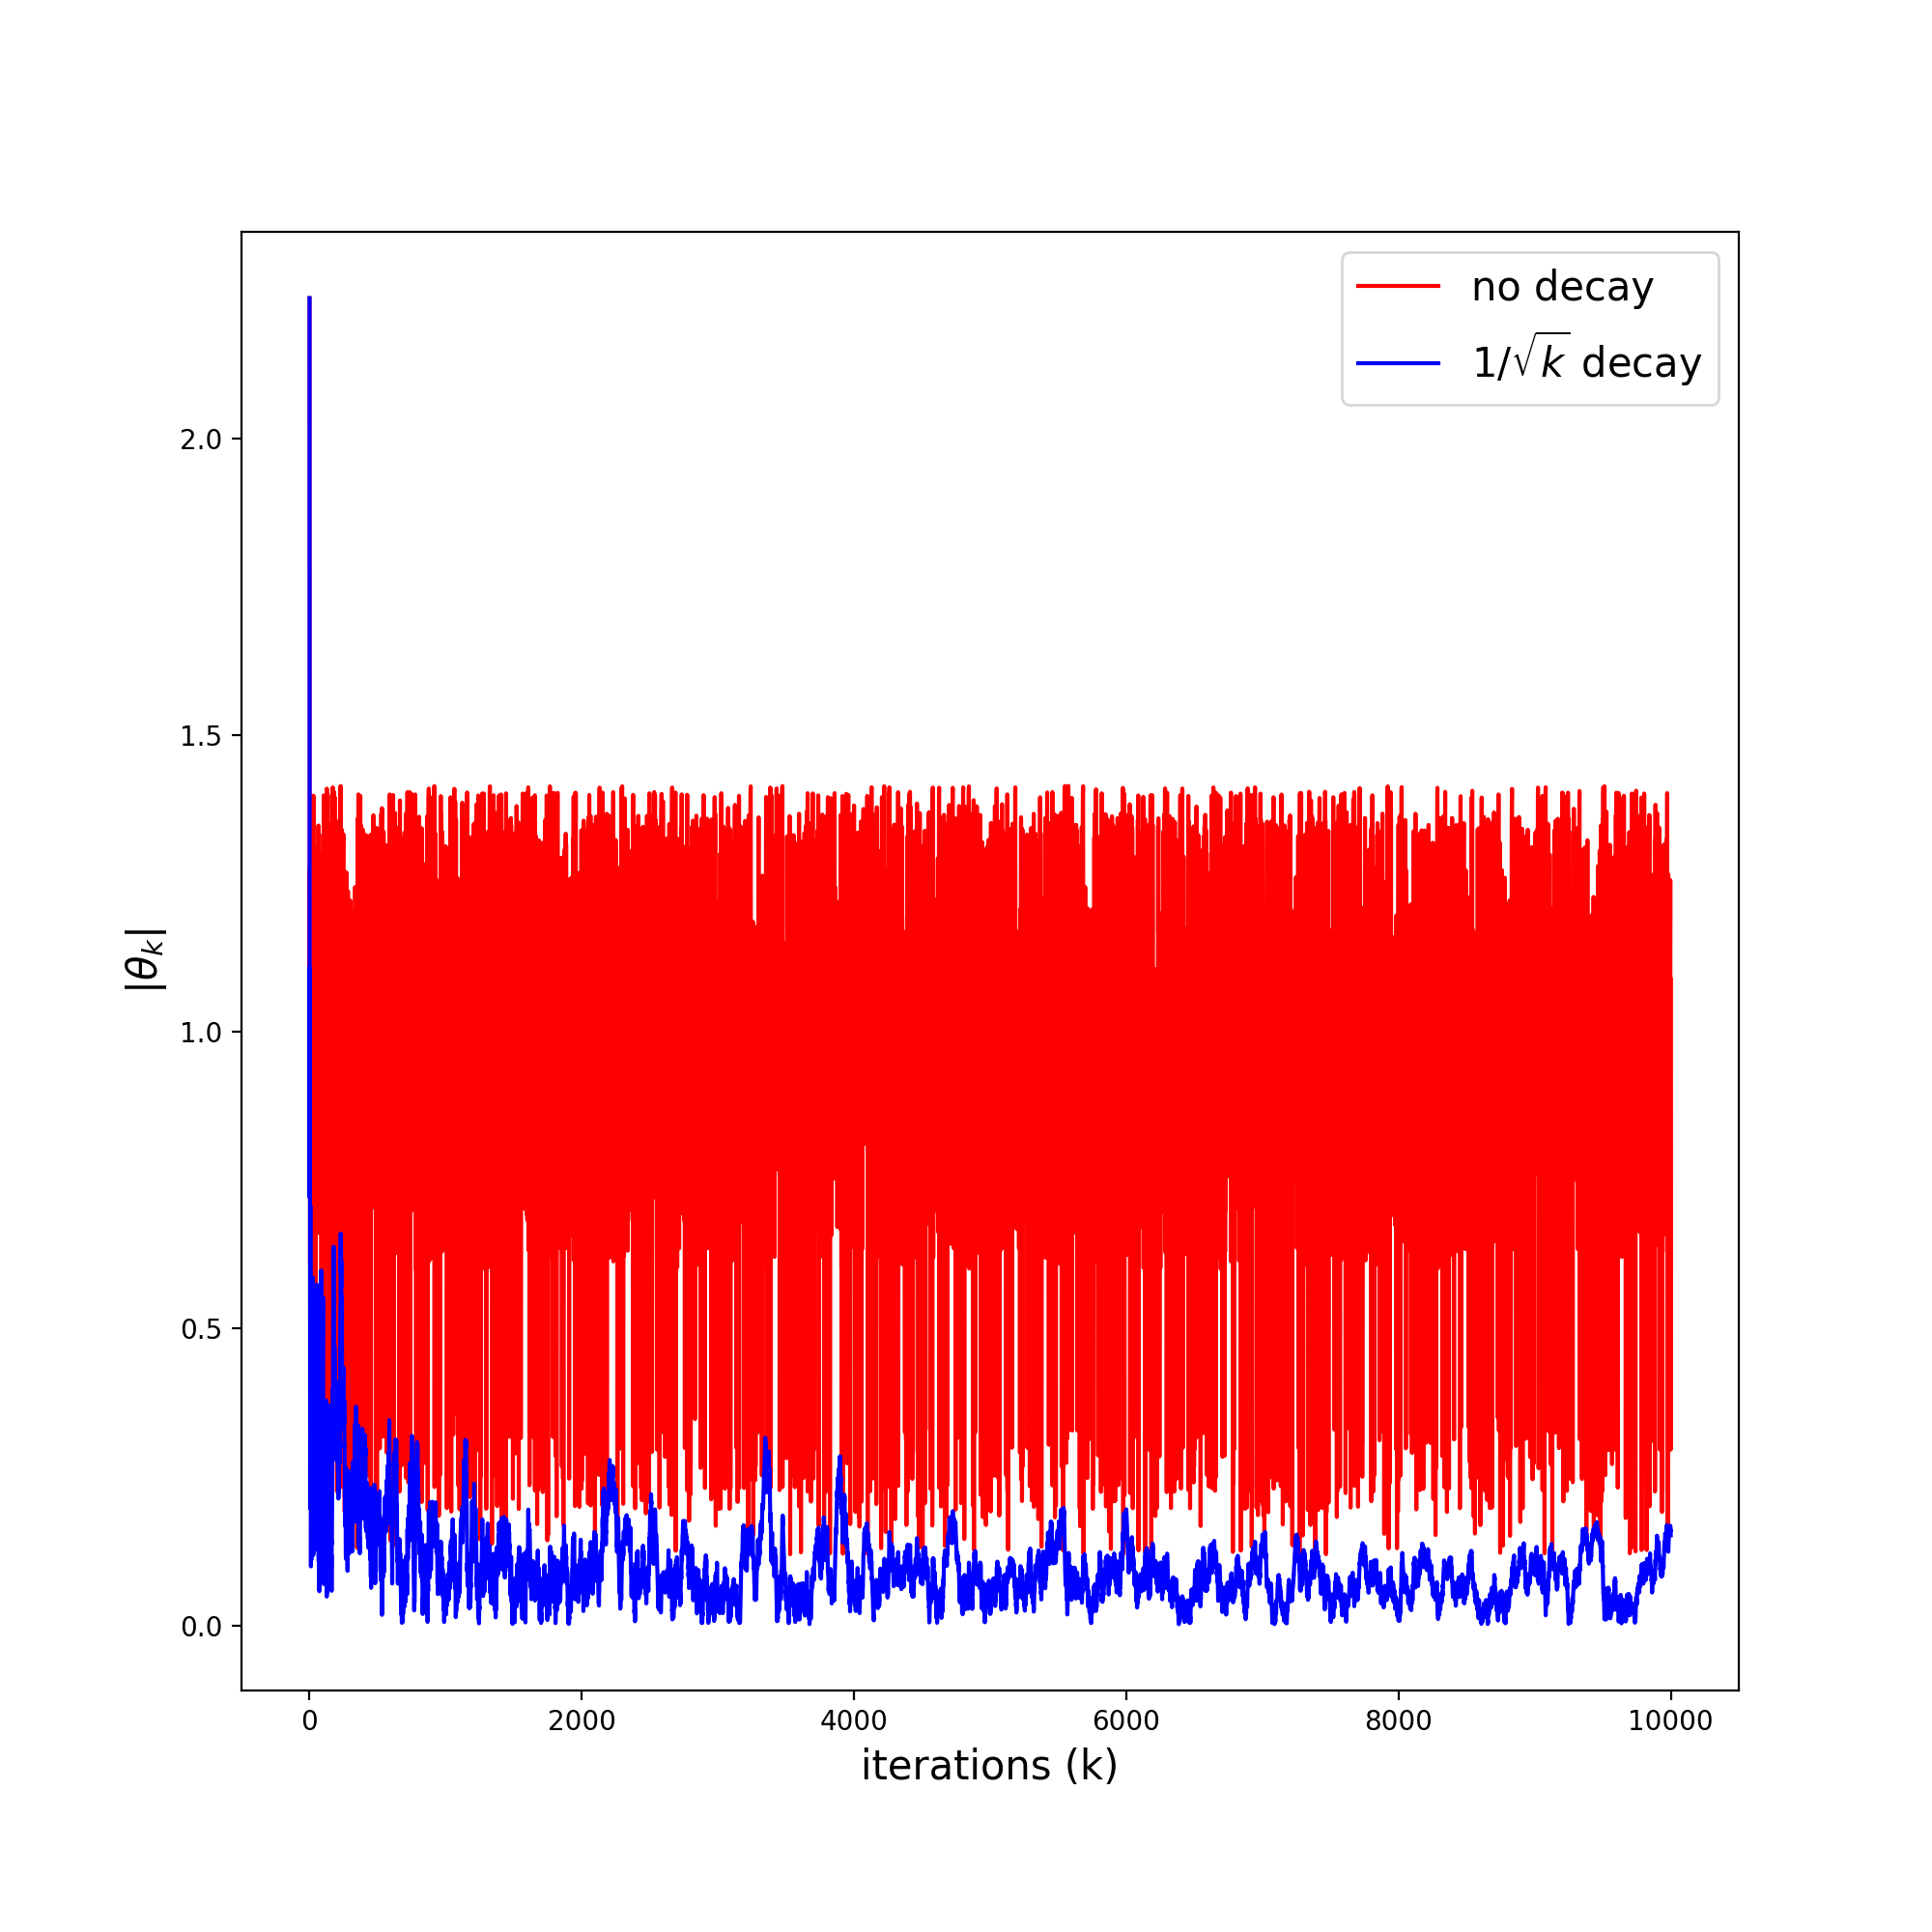
\includegraphics[width=0.45\textwidth]{fig/nn/norm_sgd.png}}
    \caption{SGD algorithm with and without a decay in the learning rate.}
    \label{fig:sgd}
  \end{center}
\end{figure}

In practice, stochastic optimization algorithms are not used for the following reasons:
\begin{enumerate}
  \item Although the loss function decays with the number of iterations, it fluctuates in a chaotic manner close the the minima and never manages to reach the minima.
  \item While handling all samples at once can be computationally expensive, handling a single sample at a time severly under-utilizes the computational and memory resources.
\end{enumerate}
However, a compromise can be made by using \textbf{mini-batch optimization}. In this strategy, the dataset of $N_\text{train}$ samples is split into $N_\text{batch}$ disjoint subsets known as mini-batches. Each mini-batch contains $\overline{N}_\text{train} = N_\text{train}/N_\text{batch}$ samples, which also refered to as the batch-size. Thus, the gradient of the loss function can be approximated by 
\begin{equation}\label{eqn:mbs_grad}
  \df{\Pi}{\btheta}(\btheta) = \frac{1}{N_\text{train}} \sum_{i=1}^{N_\text{train}} \df{\Pi_i}{\btheta}(\btheta) \approx \frac{1}{\overline{N}_\text{train}} \sum_{i \in \text{batch}(j)} \df{\Pi_i}{\btheta}(\btheta).
\end{equation}
Note that taking $N_\text{batch} = 1$ leads to the original optimization algorithms, while take $N_\text{batch} = N_\text{train}$ gives the stochastic gradient descent algorithm. One typically chooses a batch-size to maximize the amount of data that can be loaded into the RAM at one time. We define an \textbf{epoch} as one full pass through all samples (or mini-batches) of the full training set. The following describes the \text{mini-batch stochastic optimization} algorithm:
\begin{enumerate}
\item For epoch = 1, ..., J
  \begin{enumerate}
     \item Randomly shuffle the full training set
     \item Create $N_\text{batch}$ mini-batches
     \item For $ i = 1, \cdots, N_\text{batch}$
     \begin{enumerate}
        \item Evaluate the batch gradient using \eqref{eqn:mbs_grad}.
        \item Update $\btheta$ using this gradient and your favorite optimization algorithm (gradient descent, momentum, or Adam).
      \end{enumerate}   
   \end{enumerate}
\end{enumerate}

\begin{remark}
There is an interesting study \cite{WuSGD} that suggests that stochastic gradient descent might actually help in selecting minima that generalize better. In that study the authors prove that SGD prefers minima whose curvature is more homogeneous. That is, the distribution of the curvature of each of the components of the loss function is sharp and centered about a small value. This is contrast to minima where the overall curvature might be small; however the distribution of the curvature of each component of loss function is more spread out. Then they go on to show (empirically) that the more homogeneous minima tend to generalize better than their heterogeneous counterparts. 

\end{remark}

\section*{Calculating gradients using back-propagation} \label{sec:backprop}
The final piece of the training algorithm that we need to understand is how the gradients are actually evaluated while training the network. Recall the output $\vx^{(l+1)}$ of layer $l+1$ is given by
\begin{align}
  \text{Affine transform:} & \quad \xi^{(l+1)}_i= W_{ij}^{(l+1)} x_j^{(l)}+ b_i^{(l+1)}, \quad 1 \leqslant i \leqslant H_{l+1} \label{eqn:at}\\
  \text{Non-linear transform:} & \quad x^{(l+1)}_i = \sigma\left(\xi^{(l+1)}_i\right), \quad 1 \leqslant i \leqslant H_{l+1} \label{eqn:nlt}. 
\end{align}
Given a training sample $(\vx,\,\vy)$, set $\vx^{(0)} = \vx$. The value of the loss/objective function (for this particular sample) can be evaluated using the forward pass:
\begin{enumerate}
  \item For $l = 1, ..., L+1$
    \begin{enumerate}
      \item Evaluate $\xi^{(l)}$ using \eqref{eqn:at}.
      \item Evaluate $\vx^{(l)}$ using \eqref{eqn:nlt}.
    \end{enumerate}
  \item Evaluate the loss function for the given sample 
    \begin{align*}
      \Pi(\btheta) =\|\vy - \mathcal{F}(\vx; \btheta, \Hp)\|^2.
    \end{align*}   
\end{enumerate}
This operation can be written succinctly in the form of a computational graph as shown in Figure \ref{fig:comp_graph}. In this figure, the lower portion of the graph represents the evaluation of the loss function $\Pi$. 

We would of course need to repeat this step for all samples in the training set (or a mini-batch for stochastic optimization). For simplicity, we restrict the discussion to the evaluation of the loss and its gradient for a single sample.

In order to update the network parameters, we need $\df{\Pi}{\btheta}$, or more precisely $\df{\Pi}{\vW^{(l)}}$, $\df{\Pi}{\vb^{(l)}}$ for $1\leqslant l \leqslant {L+1}$. We will derive expressions for these derivatives by first deriving expressions for $\df{\Pi}{\xi^{(l)}}$ and $\df{\Pi}{\vx^{(l)}}$. 

From the computational graph it is easy to see how each hidden variable in the network is transformed to the next. Recognizing this, and applying the chain rule repeatedly yields
\begin{align}
  \df{\Pi}{\xi^{(l)}} &=  \label{eqn:dpidxi} \df{\Pi}{\vx^{(L+1)}} \cdot \df{\vx^{(L+1)}}{\xi^{(L+1)}} \cdot \df{\xi^{(L+1)}}{\vx^{(L)}} \cdots \df{\vx^{(l+1)}}{\xi^{(l+1)}} \cdot \df{\xi^{(l+1)}}{\vx^{(l)}} \cdot \df{\vx^{(l)}}{\xi^{(l)}}. 
\end{align}
In order to evaluate this expression we need to evaluate the following terms:
\begin{align}
  \df{\Pi}{\vx^{(L+1)}} &= -2 (\vy-\vx^{(L+1)})^T  \\
  \df{\xi^{(l+1)}}{\vx^{(l)}} &= \vW^{(l+1)}\\
  \df{\vx^{(l)}}{\xi^{(l)}} &= \symbfup{S}^{(l)} \equiv {\rm diag}[\sigma'(\xi^{(l)}_1), \cdots, \sigma'(\xi^{(l)}_{H_l})],
\end{align}
where the last two relations hold for any network layer $l$, $H_l$ is the width of that particular layer, and $\sigma'$ denotes the derivative of the activation with respect to its argument. Using these relations in (\ref{eqn:dpidxi}), we arrive at,
\begin{align}
  \df{\Pi}{\xi^{(l)}} &= \label{eqn:dpidxi1} \df{\Pi}{\vx^{(L+1)}} \cdot \symbfup{S}^{(L+1)} \cdot \vW^{(L+1)} \cdots \symbfup{S}^{(l+1)} \cdot \vW^{(l+1)} \cdot \symbfup{S}^{(l)}. 
\end{align}
Taking the transpose, and recognizing that $\Sigma^{(l)}$ is diagonal and therefore symmetric, we finally arrive at
\begin{align}
  \df{\Pi}{\xi^{(l)}} &= \label{eqn:dpidxifinal} \symbfup{S}^{(l)} \vW^{(l+1)T} \symbfup{S}^{(l+1)} \cdots   \vW^{(L+1)T} \symbfup{S}^{(L+1)} [-2 (\vy-\vx^{(L+1)})]. 
\end{align}
This evaluation can also be represented as a computational graph. In fact, as shown in Figure \ref{fig:comp_graph}, it can be appended to the original graph, where this part of the computation appear in the upper row of the graph. Note that we are now traversing in the backward direction.  Hence the name back propagation. 

\begin{figure}[htbp!]
\begin{center}
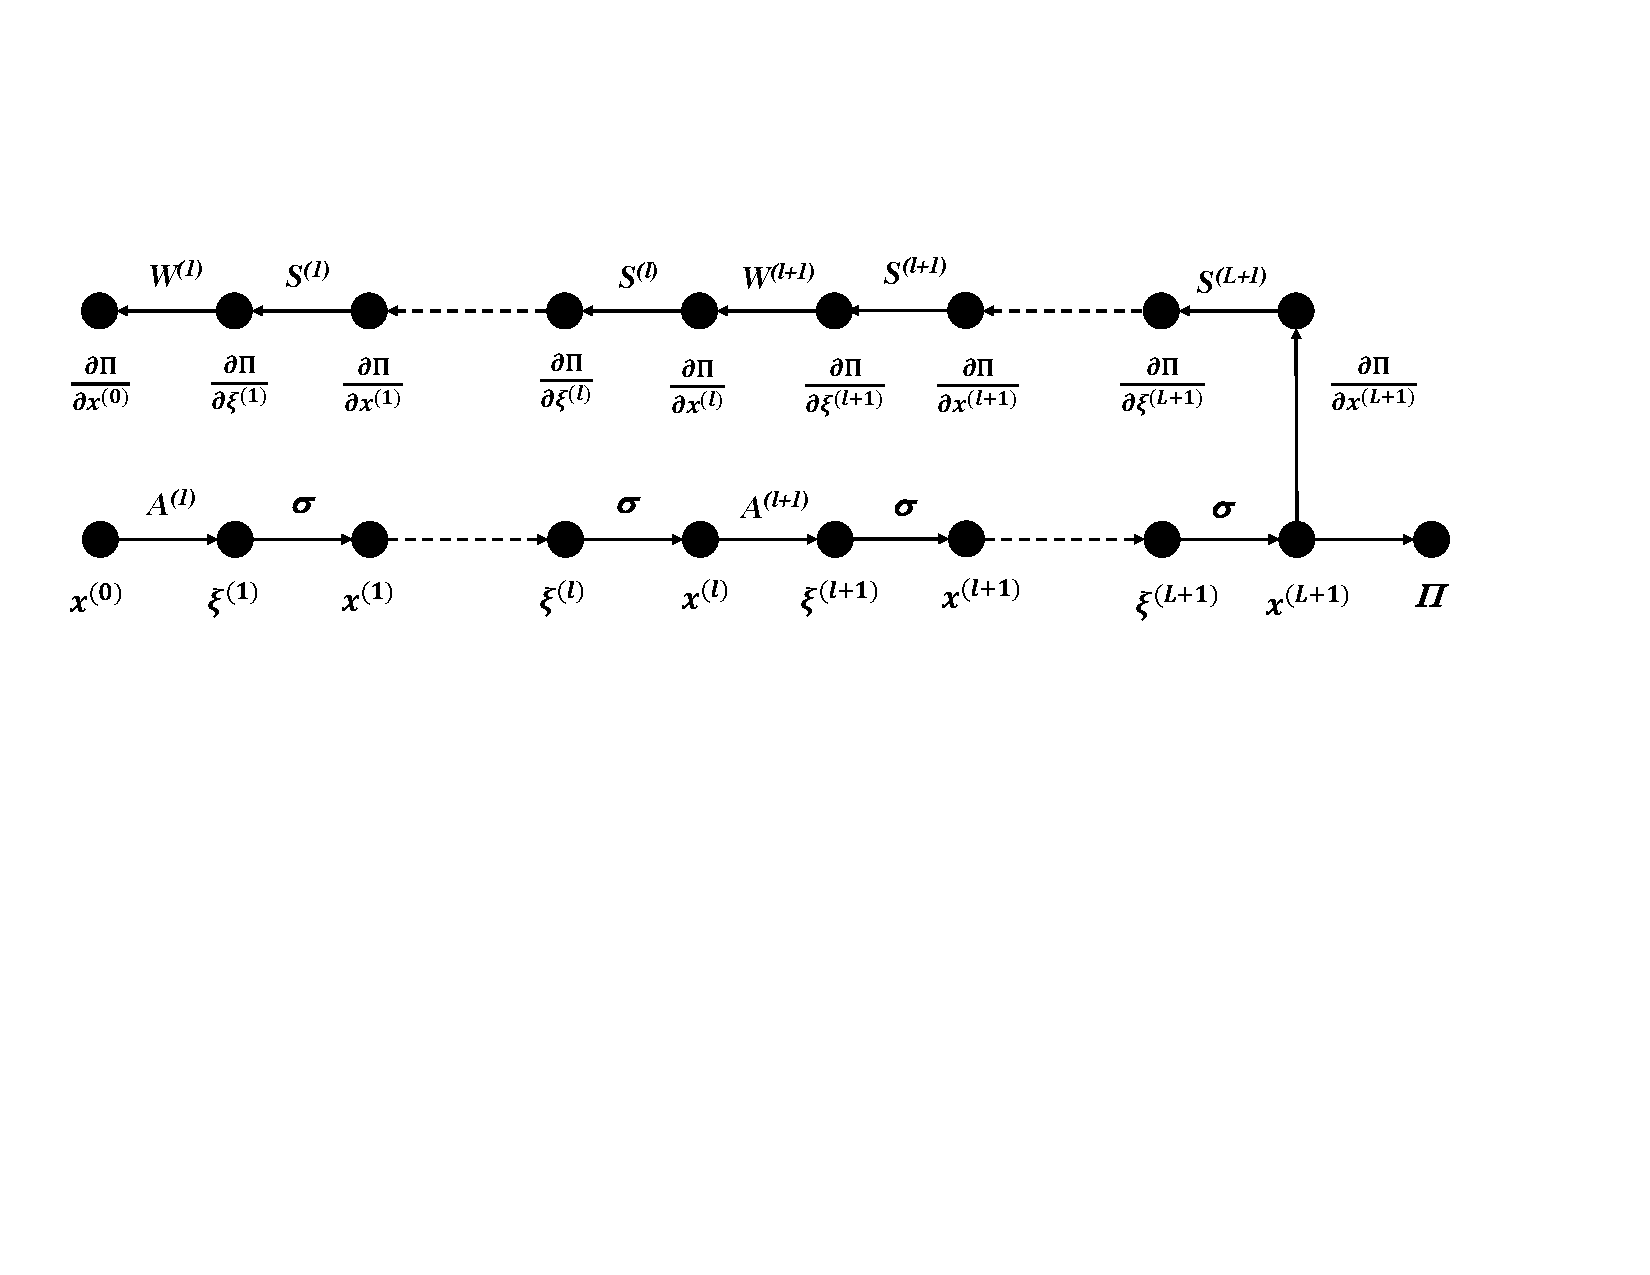
\includegraphics[width=0.90\textwidth]{fig/nn/computational_graph.pdf}
\caption{Computational graph for computing the loss function and its derivatives with respect to hidden/latent vectors.}
\label{fig:comp_graph}
\end{center}
\end{figure}

The final step is to evaluate an explicit expression for $\df{\Pi}{\vW^{(l)}}$. This can be done by recognizing,
\begin{align}\label{eqn:bpr1}
  \df{\Pi}{\vW^{(l)}} &= \df{\Pi}{\xi^{(l)}} \cdot \df{ \xi^{(l)} }{\symbfup{W}^{(l)}}  = \df{\Pi}{\xi^{(l)}} \otimes \vx^{(l-1)}, 
\end{align}
where $[\vx \otimes \vy]_{ij} = x_iy_j$  is the outer product. Thus, in order to evaluate $\df{\Pi}{\vW^{(l)}}$ we need $\vx^{(l-1)}$ which is evaluted during the forward phase and $\df{\Pi}{\xi^{(l)}}$ which is evaluated during back propagation. 

%Evaluation of these gradients will require the following relations:

%\begin{remark}
  %The $y_i$ notation in \eqref{eqn:bpr3} denotes the $i$-th component of the true output vector $\vy$, and not the $i$-th sample.
%\end{remark}

%The back-propagation algorithm to evaluate $\df{\Pi}{\vW^{(l)}}$ for each $1 \leqslant l \leqslant {L+1}$ is as follows:
%\begin{enumerate}
%  \item Evaluate $\df{\Pi}{\xi^{(L+1)}}$ using \eqref{eqn:bpr3}.
%  \item Evaluate $\df{\Pi}{\vW^{(L+1)}}$ using \eqref{eqn:bpr1} with $l = L+1$.
%  \item For $l=L,L-1,\cdots,2,1$
%    \begin{enumerate}
%      \item Evaluate $\widehat{W}_{ij}^{(l+1)}$ as defined in \eqref{eqn:bpr2}.
%      \item Evaluate $\df{\Pi}{\xi^{(l)}}$ using \eqref{eqn:bpr2}.
%      \item Evaluate $\df{\Pi}{\vW^{(l)}}$ using \eqref{eqn:bpr1}.
%    \end{enumerate}
%\end{enumerate}
%Notice, that in this algorithm the information is propagating from the outermost to the innermost layers. Just the opposite of what is done to evaluate the loss function. Thus, the part where the loss function is evaluated is called forward propagation, while the evaluation of the gradient is referred to as back-propagation. 
%Using \eqref{eqn:bpr2} repeatedly, we also have the following relation
%\begin{equation}
%  \df{\Pi}{\xi^{(l)}} = (\widehat{\vW}^{(l+1)})^\top (\widehat{\vW}^{(l+2)})^\top \cdots (\widehat{\vW}^{(L+1)})^\top \df{\Pi}{\xi^{(L+1)}}, \quad \text{for } 1 \leqslant l \leqslant L.
%\end{equation}
%Notice how the gradients are propagated backwards through the network, thus the name ``back-propagation". 

\begin{question}
  Can you derive a similar set of expressions and the corresponding algorithm to evaluate $\df{\Pi}{\vb^{(l)}}$?
\end{question}

\begin{question}
  Can you derive an explicit expression for $\df{\vx^{(L+1)}}{\vx^{(0)}}$. That is the an expression for the derivative of the output of the network with respect to its input? This is a very useful quantity that finds use in algorithms like physics informed neural networks and Wasserstein generative adversarial networks. 
\end{question}

\section*{Regression versus classification}
Till now, given the labelled dataset $\mathcal{S} = \{(\vx_i,\,\vy_i): 1 \leqslant i \leqslant N\}$, we have considered two types of losses
\begin{itemize}
  \item The mean square error (MSE)
  \begin{align*}
    \Pi(\btheta) =  \frac{1}{N_\text{train}} \sum_{i=1}^{N_\text{train}}\|\vy_i - \mathcal{F}(\vx_i; \btheta, \Hp)\|^2
  \end{align*}
  \item The mean absolute error (MAE)
  \begin{align*}
  \Pi(\btheta) =  \frac{1}{N_\text{train}} \sum_{i=1}^{N_\text{train}}\|\vy_i - \mathcal{F}(\vx_i; \btheta, \Hp)\|
  \end{align*}
\end{itemize}

Neural networks with the above losses can be used to solve various regression problems where the underlying function is highly nonlinear and the inputs/outputs are multi-dimensional.
\begin{example}
  Given the house / apartment features such as the zip code, the number of bedrooms / bathrooms, carpet area, age of construction, etc, predict the outcomes such as the market selling price, or the number of days on the market.
\end{example}

Now let us consider some examples of classification problems, where the output of the network typically lies in a discrete finite set.
\begin{example}
  Given the symptoms and blood markers of patients with COVID-19, predict whether they will need to be admitted to ICU. So the input and output for this problem would be
  \begin{equation*}
    \begin{aligned}
    \vx &= [\text{pulse rate},\,\text{temperature},\,\text{SPO}_2,\,\text{procalcitonin},\,... ]\\
    \vy &= [p_1,\,p_2]
    \end{aligned}
  \end{equation*}
  where $p_1$ is the probability of being admitted to the ICU, while $p_2$ is the probability of not being admitted. Note that $0 \leqslant p_1, p_2 \leq1$ and $p_1 + p_2 = 1$.
\end{example}

\begin{example}\label{ex:3class}
Given a set of images of animals, predict whether the animal is a dog, cat or bird. In this case, the input and output should be
\begin{equation*}
  \begin{aligned}
  \vx &= \text{the image}\\
  \vy &= [p_1,p_2,p_2]
  \end{aligned}
\end{equation*}
where $p_1,p_2,p_3$ is the probability of being a dog, cat or bird, respectively.
\end{example}

Since the output for the classification problem corresponds to probabilities, we need to make a few changes to the network
\begin{enumerate}
  \item Make use of an output function at the end of the output layer that suitably transforms the output vector into the desired form, i.e, a vector of probabilities. This is typically done using the \textbf{softmax function}
  \begin{align*}
    x_i^{(L+1)} = \frac{\exp{(\xi_i^{(L+1)})}}{\sum_{j=1}^C\exp{(\xi_j^{(L+1)})}}
  \end{align*}
  where $C$ is the number of classes (and also the output dimension). Verify that with this transformation, the components of the $\vx^{(L+1)}$ form a convex combination, i.e., $x_i^{(L+1)} \in [0,1]$ and $\sum_{i=1}^C x_i^{(L+1)} = 1$.
  \item The output labels for the various samples need to be one-hot encoded. In other words, for the sample $(\vx, \vy)$, the output label $\vy$ should have dimension $D=C$, and whose component is 1 only for the component signifying the class $\vx$ belongs  to, otherwise 0. For instance, in Example \ref{ex:3class} 
  \begin{align*}
    \vy = \begin{cases}
      [1,\,0,\,0]^\top & \quad \text{if $\vx$ is a dog},\\ 
      [0,\,1,\,0]^\top & \quad \text{if $\vx$ is a cat},\\
      [0,\,0,\,1]^\top & \quad \text{if $\vx$ is a pig}.
    \end{cases}
  \end{align*}

  \item Although the MSE or MSA can still be used as the loss function, it is preferable to use the \text{cross-entropy} loss function
    \begin{equation}\label{eqn:crossentropy}
      \Pi(\btheta) = \frac{1}{N_\text{train}} \sum_{i=1}^{N_\text{train}} \sum_{c=1}^{C} - y_{ci} \log(\mathcal{F}_{\!\!\!c}(\vx_i;\btheta)),
    \end{equation}
    where $y_{ci}$ is the $c$-th component of the true label for the $i$-th sample.
    The loss function in \eqref{eqn:crossentropy} treats $y_c$ and $\mathcal{F}_{\!\!\!c}$ as probability distributions and measures the discrepancy between the two. It can be shown to be related to the Kullback-Liebler divergence between the two distributions. Compared to MSE, this loss function severely penalizes strongly confident incorrect predictions. This is demonstrated in Example \ref{ex:cr_ent}
\end{enumerate}

\begin{example}\label{ex:cr_ent}
  Let us consider a binary classification problem, i.e., $C=2$. For a given $\vx$, let $\vy = [0,1]$ and let the prediction be $\mathcal{F} = [p, 1-p]$. Clearly, a small value of $p$ is preferred. Therefore any reasonable cost function should penalize large values of $p$. Now let us evaluate the error using various loss functions
\begin{itemize}
  \item MSE Loss $\ds= (0-p)^2 + (1 - 1 +p)^2 = 2p^2$.
  \item Cross-entropy Loss $\ds= -(0 \log(p) + 1 \log(1-p) = - \log(1-p)$.
\end{itemize}
Note that both losses penalize large values of $p$. Also when $p = 0$, both losses are zero. However, as $p \to 1$ (which would lead the wrong prediction), the MSE loss $\to 2$, while the cross-entropy loss $\to \infty$. That is, it strongly penalizes incorrect confident predictions. 
\end{example}

\bibliographystyle{elsarticle-harv}
\bibliography{note10}

\end{document}
